\chapter{The concept of black hole}

\minitoc

\section{Introduction}

%%%%%%%%%%%%%%%%%%%%%%%%%%%%%%%%%%%%%%%%%%%%%%%%%%%%%%%%%%%%%%%%%%%%%%%%%%%%%%%%%%%%%%%%


\section{Black holes and null hypersurfaces}

\subsection{A first definition of black holes} \label{s:def:first_defin}

A naive definition of a black hole, involving only words, could be
\begin{quote}
A \defin{black hole}\index{black!hole} is a localized region of spacetime
from which neither massive particles nor massless ones (photons) may escape.
\end{quote}
There are essentially two features in this definition: \emph{localization}
and \emph{inescapability}. Let us for a moment focus on the latter.
It implies the existence of a \emph{boundary}, which no
particle emitted in the black hole region can cross.
This boundary is called the
\defin{event horizon}\index{event!horizon}\index{horizon!event --} and is
quite often referred to simply as the \defin{horizon}.
It is a \defin{one-way membrane}\index{one-way membrane}\index{membrane!one-way --},
in the sense that it can be crossed from the black hole ``exterior'' towards
the black hole region, but not in the reverse way. The one-way membrane must be
a hypersurface of the spacetime manifold $\M$, for it has to divide $\M$ in two regions:
the interior (the black hole itself) and the exterior region.
Let us recall that a hypersurface is a submanifold of $\M$ of codimension 1
(cf. Sec.~\ref{s:bas:embed} in Appendix~\ref{s:bas}).

\subsection{The event horizon as a null hypersurface}

To discuss further which hypersurface could act as a black hole boundary,
one should recall that, on a Lorentzian manifold $(\M,\w{g})$, there are
three classes of hypersurfaces. The classification
depends on the type of metric induced by $\w{g}$ on the
hypersurface, $\Sigma$ say, the
\defin{induced metric}\index{induced!metric}\index{metric!induced --} being
nothing but the restriction $\left.\w{g}\right| _{\Sigma}$ of $\w{g}$
to vector fields tangent to $\Sigma$.
A hypersurface $\Sigma$ is said to be
\begin{itemize}
\item \defin{spacelike} iff $\left.\w{g}\right| _{\Sigma}$ is positive definite,
i.e. iff $\mathrm{sign} \left.\w{g}\right| _{\Sigma} = (+,+,+)$,
i.e. iff $(\Sigma,  \left.\w{g}\right| _{\Sigma})$ is a Riemannian manifold;
\item \defin{timelike} iff $\left.\w{g}\right| _{\Sigma}$ is a Lorentzian metric,
i.e. iff $\mathrm{sign} \left.\w{g}\right| _{\Sigma} = (-,+,+)$,
i.e. iff $(\Sigma,  \left.\w{g}\right| _{\Sigma})$ is a Lorentzian manifold;
\item \defin{null} iff $\left.\w{g}\right| _{\Sigma}$ is degenerate\footnote{
Cf. Sec.~\ref{s:bas:metric} in Appendix~\ref{s:bas} for the definition of a
degenerate bilinear form; the degeneracy
implies that the bilinear form $\left.\w{g}\right| _{\Sigma}$ is not,
strictly speaking, a metric on $\Sigma$.}
i.e. iff $\mathrm{sign} \left.\w{g}\right| _{\Sigma} = (0,+,+)$.
\end{itemize}
The hypersurface type can also be deduced from the normal vector
$\w{n}$ to it (cf. Sec.~\ref{s:bas:hyp_normal}):
\begin{itemize}
\item $\Sigma$ spacelike $\iff$ $\w{n}$ timelike;
\item $\Sigma$ timelike $\iff$ $\w{n}$ spacelike;
\item $\Sigma$ null $\iff$ $\w{n}$ null.
\end{itemize}
These equivalences are easily proved by considering a $\w{g}$-orthogonal basis
adapted to $\Sigma$.

\begin{remark}
Null hypersurfaces have the distinctive feature that their normals are
also tangent to them. Indeed, by definition, the normal $\w{n}$ is null iff
$\w{n}\cdot\w{n}=0$, which is nothing but the condition
for $\w{n}$ to be tangent to $\Sigma$.
\end{remark}

Only null and spacelike hypersurfaces are eligible as a one-way membrane
regarding timelike and null worldlines (cf. Fig.~??).
The limit case between two-way membranes (timelike hypersurfaces)
and one-way ones being null hypersurfaces, it is quite natural to select the
latter ones for the black hole boundary, rather than spacelike hypersurfaces.
Note however that in Chap.~??, we shall see that spacelike hypersurfaces,
called \emph{dynamical
horizons}\index{dynamical!horizon}\index{horizon!dynamical --}, are involved
in the quasi-local approaches to black holes.

%%%%%%%%%%%%%%%%%%%%%%%%%%%%%%%%%%%%%%%%%%%%%%%%%%%%%%%%%%%%%%%%%%%%%%%%%%%%%%%%

\section{Geometry of null hypersurfaces}

Having decided that the black hole event horizon must be a null hypersurface,
let us examine the geometrical properties of such a hypersurface. We shall
denote it by $\Hor$, for \emph{horizon}, but the results of this section
will be valid for any null hypersurface.

\subsection{Null generators} \label{s:def:null_gener}

As any hypersurface, $\Hor$ can be locally considered as a level set,
around any point of $\Hor$, there exists an open subset $\mathscr{U}$
of $\M$ (possibly  $\mathscr{U} = \M$) and
a smooth scalar field $u:\ \mathscr{U} \rightarrow \R$ such that
\be \label{e:def:Hor_u_zero}
    \forall p \in \mathscr{U},\quad p\in \Hor \iff u(p) = 0 .
\ee
\begin{example}[null hyperplane] \label{x:def:null_hyp}
A very simple example of null hypersurface is a null hyperplane in
the 4-dimensional Minkowski spacetime. If $(t,x,y,z)$ are standard Minkowskian
coordinates, the choice of the scalar field
\be \label{e:def:null_plane_u}
    u(t,x,y,z) = t - x
\ee
defines a null hyperplane by $u=0$.
\end{example}

\begin{example}[light cone] \label{x:def:light_cone}
Another simple example of null hypersurface, still in the 4-dimensional Minkowski spacetime,
is the future sheet $\Hor$ of a light cone\index{light!cone}\index{cone!light --}, also
called \defin{future light cone}\index{future!light cone}. Note that we have
to take out the apex from $\Hor$, in order to have a regular hypersurface.
In the  Minkowskian coordinates $(t,x,y,z)$, the choice of the
``retarded time''\index{retarded!time}
\be \label{e:def:light_cone_u}
    u(t,x,y,z) = t - \sqrt{x^2+y^2+z^2}
\ee
defines a future light cone by $u=0$.
\end{example}

\begin{example}[Schwarzschild horizon] \label{x:def:Schw_hor}
Let us consider the 4-dimensional spacetime $(\M,\w{g})$ with $\M$ diffeomorphic
to $\mathbb{R}^4$ and equipped with a coordinate system $(x^\alpha)=(t,r,\th,\ph)$
($t\in \mathbb{R}$, $r\in(0,+\infty)$, $\th\in(0,\pi)$
and $\ph\in(0,2\pi)$) such that $\w{g}$ takes the form
\be \label{e:def:Schw_metric}
    g_{\mu\nu} \D x^\mu \D x^\nu = - \left( 1 - \frac{2 m}{r} \right) \D t^2
        + \frac{4m}{r} \, \D t \, \D r
        + \left( 1 + \frac{2 m}{r} \right) \D r^2
        + r^2\D\th^2 + r^2\sin^2\th \, \D\ph^2 ,
\ee
where $m$ is a positive constant. We shall see in Chap.~\ref{s:sch} that
$(\M,\w{g})$ is actually a part of Schwarzschild spacetime, described in
coordinates different from the standard ones,  $(\bar t, r, \th, \ph)$
say, by the choice of the time coordinate:
$t = {\bar t} + 2m\ln|r/(2m)-1|$. The present coordinates are called
\defin{3+1 Eddington-Finkelstein coordinates}\index{Eddington-Finkelstein!coordinates}
and have the advantage over the the standard ones to be regular on the event horizon,
which is located at $r=2m$. Indeed, the metric components (\ref{e:def:Schw_metric})
remain finite when $r\rightarrow 2m$, as those of the inverse metric, which are
\be \label{e:def:Schw_metric_inv}
    g^{\alpha\beta} = \left(
    \begin{array}{cccc}
    - 1 - \frac{2m}{r} & \frac{2m}{r} & 0 & 0 \\
    \frac{2m}{r} & 1 - \frac{2m}{r} & 0 & 0 \\
    0 & 0 & \frac{1}{r^2} & 0 \\
    0 & 0 & 0 & \frac{1}{r^2\sin^2\th}
    \end{array} \right) .
\ee
Let us consider the scalar field defined on $\M$ by
\be \label{e:def:Schw_u}
    u(t,r,\th,\ph) = \left( 1 - \frac{r}{2m} \right)
            \exp\left(\frac{r-t}{4m}\right) .
\ee
It is then clear that the hypersurface $u=0$ is the
3-dimensional ``cylinder'' $\Hor$ of equation
$r=2m$. We shall see below\footnote{This should be obvious for the experienced
reader since a normal 1-form to $\Hor$ is $\dd r$ and, from Eq.~(\ref{e:def:Schw_metric_inv}), $g^{rr}=0$ on $\Hor$.} that $\Hor$ is indeed a null hypersurface.
\end{example}

Let $\wl$ be a vector field normal to $\Hor$. Since $\Hor$ is a null hypersurface,
$\wl$ is a null vector:
\be \label{e:def:wl_null}
    \wl\cdot\wl = 0
\ee
\begin{remark}
As a consequence of (\ref{e:def:wl_null}), there is no natural normalization
of $\wl$, contrary to the case of timelike or spacelike hypersurfaces,
where one can always choose the normal to be a unit vector
(scalar square equal to $1$ or $-1$). It follows that there is no unique choice
of $\wl$. At this stage, any rescaling $\wl \mapsto \wl' =  \alpha \wl$, with
$\alpha$ a strictly positive (or strictly negative) scalar field on $\Hor$,
yields a normal vector field $\wl'$ as valid as $\wl$.
\end{remark}
The null normal vector field $\wl$ is a priori defined on $\Hor$
only and not at points $p\not\in\Hor$.
However, it is worth to consider $\wl$ as a vector field
not confined to $\Hor$ but defined
in some open subset of $\M$ around $\Hor$.
In particular this would permit to define the spacetime covariant
derivative $\w{\nabla}\wl$, which is not possible if the
support of $\wl$ is restricted to $\Hor$.
Following Carter \cite{Carte97}, a simple way to achieve
this is to consider not only a single null hypersurface $\Hor$,
but a foliation of $\M$ (in the vicinity
of $\Hor$) by a family of null hypersurfaces, such that $\Hor$ is an
element of this family.
Without any loss of generality,
we may select the value of the scalar field $u$ to label these hypersurfaces and
denote the family by $(\Hor_u)$. The null hypersurface $\Hor$
is then nothing but the element $\Hor = \Hor_{u=0}$ of this family
[Eq.~(\ref{e:def:Hor_u_zero})].
The vector field $\wl$ can then be viewed as defined in the part of $\M$
foliated by $(\Hor_u)$, such that at each point in this region, $\wl$
is null and normal to $\Hor_u$ for some value of $u$.

\begin{example}
The scalar field $u$ introduced in Example~\ref{x:def:null_hyp}
(null hyperplane) does define a family of null hypersurfaces
$(\Hor_u)$. A counter-example would be $u(t,x,y,z)=(t-x)(1+x^2)$, since
$u=a$ does not define a null hypersurface except for $a=0$.
Similarly, the scalar fields $u$ of
Example~\ref{x:def:light_cone} (light cone)
and Example~\ref{x:def:Schw_hor} (Schwarzschild horizon)
do define a family of null
hypersurfaces $(\Hor_u)$. In the latter example, this would not have been the
case for the simpler choice $u(t,r,\th,\ph)  = r - 2m$.
\end{example}

Obviously the family $(\Hor_u)$ is non-unique but all geometrical
quantities that we shall introduce hereafter do not depend upon the choice
of the foliation $\Hor_u$ once they are evaluated at $\Hor$.

Since $\Hor$ is a hypersurface where $u$ is constant [Eq.~(\ref{e:def:Hor_u_zero})],
we have, by definition,
\bea
    \forall \w{v}\in T_p\M,\quad \w{v} \mbox{\ tangent to\ }\Hor & \iff  & \langle \wnab u , \w{v} \rangle = 0 \nonumber \\
    & \iff & \vw{\nabla} u \cdot \w{v} = 0 ,   \label{e:def:nab_u_normal}
\eea
where $\vw{\nabla} u$ is the gradient vector field of the scalar field $u$.
Property (\ref{e:def:nab_u_normal}) means that $\vw{\nabla} u$ is
a normal vector field to $\Hor$. By uniqueness of the normal direction, it
must then be colinear to $\wl$. Therefore, there must exist some scalar
field $\rho$ such that
\be \label{e:def:wl_rho_u}
    \encadre{\wl = - e^\rho \, \vw{\nabla} u } .
\ee
We have chosen the
coefficient linking $\wl$ and $\vw{\nabla} u $ to be strictly negative,
i.e. under the form of minus an exponential. This is always possible by a suitable
choice of the scalar field $u$. The minus sign ensures that in the case
of a retarded time $u$ increasing toward the future, $\wl$ is future-directed.

\begin{example}[null hyperplane] \label{x:def:null_hyp2}
We deduce from the
expression (\ref{e:def:null_plane_u}) chosen for $u$ in Example~\ref{x:def:null_hyp} that
\[
    \wnab u = \dd t - \dd x .
\]
The gradient vector field obtained by metric duality is
$\vw{\nabla} u = - \wpar_t - \wpar_x$. Choosing for simplicity $\rho=0$,
we get from formula~(\ref{e:def:wl_rho_u})
\be \label{e:def:wl_null_hyperplane}
    \wl =  \wpar_t + \wpar x .
\ee
\end{example}

\begin{example}[light cone] \label{x:def:light_cone2}
Regarding Example~\ref{x:def:light_cone}, we have,
given expression (\ref{e:def:light_cone_u}) for $u$,
\[
    \wnab u = \dd t - \frac{x}{r} \dd x - \frac{y}{r} \dd y - \frac{z}{r} \dd z,
    \quad\mbox{with}\quad r:=\sqrt{x^2+y^2+z^2}.
\]
Choosing for simplicity $\rho=0$ in (\ref{e:def:wl_rho_u}), we get the
normal
\be \label{e:def:wl_light_cone}
    \wl = \wpar_t + \frac{x}{r} \wpar_x + \frac{y}{r} \wpar_y + \frac{z}{r} \wpar_z .
\ee
\end{example}

\begin{example}[Schwarzschild horizon] \label{x:def:Schw_hor2}
We deduce from the expression (\ref{e:def:Schw_u}) chosen for $u$ in
Example~\ref{x:def:Schw_hor} that
\[
    \wnab u = \frac{1}{4 m} \mathrm{e}^{(r-t)/(4m)} \left[ - \left(1-\frac{r}{2m}  \right)
        \, \dd t
        - \left(1 + \frac{r}{2m}\right) \, \dd r \right] .
\]
The corresponding gradient vector field, $\nabla^\alpha u = g^{\alpha\mu} \nabla_\mu u$,
is computed from the expression
(\ref{e:def:Schw_metric_inv}) of $g^{\alpha\mu}$:
\[
    \vw{\nabla} u = \frac{1}{4 m} \mathrm{e}^{(r-t)/(4m)} \left[
    - \left(1+ \frac{r}{2m} \right) \wpar_t
    + \left(1 - \frac{r}{2m} \right) \wpar_r \right] .
\]
This time, we do not chose $\rho=0$ but rather select $\rho$ so that
$\el^t = 1$:
\[
    e^\rho =  - \frac{1}{\nabla^t u} \iff
    \rho = \frac{t-r}{4m} - \ln \left( 1 + \frac{r}{2m} \right) + \ln (4 m).
\]
Equation~(\ref{e:def:wl_rho_u}) then leads to
\be \label{e:def:wl_Schw_hor}
    \wl = \wpar_t + \left( \frac{r-2m}{r+2m} \right) \wpar_r .
\ee
Given the metric (\ref{e:def:Schw_metric}), we check that $\w{g}(\wl, \wl)=0$.
Since $\wl\not=0$, this proves that all hypersurfaces $\Hor_u$, and in particular $\Hor$,
are null.

\end{example}

\subsubsection{Frobenius identity}

Let us take the metric dual of relation (\ref{e:def:wl_rho_u}): it writes
$\uu{\el} = - e^\rho \, \wnab u$, or, in index notation,
\be
    \el_\alpha = - e^\rho \, \nabla_\alpha u .
\ee
Taking the covariant derivative, we get
\[
    \nabla_\alpha \el_\beta = - e^\rho \nabla_\alpha \rho \nabla_\beta u
                -   e^\rho  \nabla_\alpha \nabla_\beta u
                 = \nabla_\alpha \rho \, \el_\beta - e^\rho  \nabla_\alpha \nabla_\beta u
\]
Antisymmetrizing and using the torsion-free property of $\wnab$ (i.e.
$\nabla_\alpha \nabla_\beta u - \nabla_\beta \nabla_\alpha u = 0$, cf.
Eq.~(\ref{e:bas:torsion-free}) in Appendix~\ref{s:bas}), we get
\be \label{e:def:ext_der_wl_comp}
  \nabla_\alpha \el_\beta - \nabla_\beta \el_\alpha =
  \nabla_\alpha \rho \, \el_\beta -  \nabla_\beta \rho \, \el_\alpha  .
\ee
In the left-hand side there appears the exterior derivative of
the 1-form $\uu{\el}$ (cf. Sec.~\ref{s:bas:ext_deriv} in Appendix~\ref{s:bas}),
while one recognize in the right-hand side the exterior product of
the two 1-forms $\dd\rho$ and $\uu{\el}$. Hence we may rewrite (\ref{e:def:ext_der_wl_comp})
as
\be
    \encadre{ \dd \uu{\el} = \dd\rho \wedge \uu{\el} } .
\ee
This reflects the \defin{Frobenius theorem}\index{Frobenius!theorem}
in its dual formulation (see e.g.
Theorem B.3.2 in Wald's textbook \cite{Wald84}): the exterior derivative of
the 1-form $\uu{\el}$ is the exterior product of $\uu{\el}$ itself with some
1-form ($\dd\rho$ in the present case) if, and only if,
$\uu{\el}$ defines hyperplanes that are integrable in some hypersurface ($\Hor$ in the present case).

\subsubsection{Geodesic generators}

Let us contract the Frobenius identity (\ref{e:def:ext_der_wl_comp}) with $\wl$:
\be \label{e:def:l_contract_Frob}
    \el^\mu \nabla_\mu \el_\alpha - \el^\mu \nabla_\alpha \el_\mu
        = \el^\mu \nabla_\mu \rho \, \el_\alpha
        - \underbrace{\el^\mu \el_\mu}_{0} \nabla_\alpha \rho .
\ee
Now, since $\wl$ is a null vector,
\[
    \el^\mu \nabla_\alpha \el_\mu = \nabla_\alpha (\underbrace{\el^\mu \el_\mu}_{0})
        - \el_\mu \nabla_\alpha \el^\mu ,
\]
from which we get
\be \label{e:def:el_nab_el_zero}
    \el^\mu \nabla_\alpha \el_\mu = 0 .
\ee
Hence (\ref{e:def:l_contract_Frob}) reduces to
\be \label{e:def:wl_geod_kappa_dual}
    \el^\mu \nabla_\mu \el_\alpha  = \kappa \, \el_\alpha ,
\ee
with
\be \label{e:def:def_kappa}
    \kappa := \el^\mu \nabla_\mu \rho = \wnab_{\wl}\,  \rho .
\ee
The metric dual of (\ref{e:def:wl_geod_kappa_dual}) is
\be \label{e:def:wl_geod_kappa}
    \encadre{ \wnab_{\wl}\, \wl = \kappa \, \wl } .
\ee
This equation implies that the field lines of $\wl$ are geodesics.
To demonstrate this, we note that a rescaling
\be \label{e:def:wl_rescale}
    \wl \mapsto \wl' =  \alpha \wl
\ee
with $\alpha$ a strictly positive scalar field can be performed to yield
a geodesic vector field\index{geodesic!vector field} $\wl'$, i.e.
a vector field that obeys
\be
    \wnab_{\wl'}\, \wl' = 0 .
\ee
Indeed, Eqs.~(\ref{e:def:wl_rescale}) and
(\ref{e:def:wl_geod_kappa}) imply
\be \label{e:def:nab_lp_lp}
    \wnab_{\wl'}\, \wl' = \alpha\left(
        \wnab_{\wl}\, \alpha + \kappa \alpha \right) \wl .
\ee
Hence, since $\alpha>0$,
\[
    \wnab_{\wl'}\, \wl' = 0  \iff  \wnab_{\wl}\, \ln \alpha = -\kappa .
\]
Therefore it suffices to solve $\wnab_{\wl}\, \ln \alpha = -\kappa$, which
is a first-order ordinary differential equation along each field line of $\wl$
to ensure that $\wl'$ is a geodesic vector field.
The field lines of $\wl'$ are then null geodesics and $\wl'$ is the tangent
vector to them associated with some affine parameter $\lambda$.
On the other side, if $\kappa\not=0$, $\wl$ is not a geodesic vector field
and therefore cannot be associated with some affine parameter. For this
reason the quantity $\kappa$ is called the
\defin{non-affinity parameter}\index{non-affinity parameter} of
the null normal $\wl$.

Since $\wl$ is colinear to $\wl'$, it obviously share the same field lines.
These field lines are called the
\defin{null generators}\index{null!generator}\index{generator!of a null hypersurface}
of the hypersurface $\Hor$.

Hence, we have shown that
\begin{quote}
Any null hypersurface $\Hor$ is ruled by a family of null geodesics, called the
null generators, and each vector field $\wl$ normal to $\Hor$ is
tangent to these null geodesics.
\end{quote}
As a by-product of (\ref{e:def:nab_lp_lp}), we get the behavior of the
non-affinity parameter under a rescaling of the null normal:
\be \label{e:def:rescale_kappa}
    \wl' = \alpha \wl \ \Longrightarrow \ \kappa' = \alpha \kappa + \wnab_{\wl} \alpha .
\ee

\begin{example}[null hyperplane] \label{x:def:null_hyp3}
It is clear on expression (\ref{e:def:wl_null_hyperplane}) for $\wl$ that
the covariant derivative
$\wnab \wl$ vanishes identically. In particular $\wnab_{\wl} \wl = 0$.
Equation~(\ref{e:def:wl_geod_kappa}) then implies
\[
    \kappa = 0 ,
\]
which is in agreement with Eq.~(\ref{e:def:def_kappa}) and the choice $\rho=0$
performed in Example~\ref{x:def:null_hyp2}. The null generators of $\Hor$ are the
straight lines defined by $t=x$, $y=y_0$ and $z=z_0$ for some constants
$(y_0,z_0)\in \mathbb{R}^2$. Either $t$ or $x$ can be chosen as an affine
parameter of these generators.
\end{example}

\begin{example}[light cone] \label{x:def:light_cone3}
We get from the expression (\ref{e:def:wl_light_cone})
of $\wl$ and the fact that in Minkowksi coordinates $(t,x,y,z)$,
$\nabla_\beta \el^\alpha = \partial_\beta \el^\alpha$,
\be \label{e:def:nab_l_light_cone}
    \nabla_\beta \el^\alpha = \left(
    \begin{array}{cccc}
    0 & 0 & 0 & 0 \\
    0 & \frac{y^2+z^2}{r^3} & - \frac{xy}{r^3} & - \frac{xz}{r^3} \\
    0 & - \frac{xy}{r^3} & \frac{x^2+z^2}{r^3} & - \frac{yz}{r^3} \\
    0 & - \frac{xz}{r^3} & - \frac{yz}{r^3} & \frac{x^2+y^2}{r^3}
    \end{array} \right)
    \qquad {(\alpha = \mbox{row index}; \atop \beta = \mbox{column index}).}
\ee
We obtain then $\el^\mu \nabla_\mu \el^\alpha = 0$.
From Eq.~(\ref{e:def:wl_geod_kappa}), we conclude that
\[
    \kappa = 0 ,
\]
which is in agreement with Eq.~(\ref{e:def:def_kappa}) and the choice $\rho=0$
performed in Example~\ref{x:def:light_cone2}. The null generators of $\Hor$
are the half-lines defined by $x=a t$, $y=b t$, $z = \sqrt{1-a^2-b^2} t$, with
$t>0$ and $(a,b)\in\mathbb{R}^2$ such that $a^2+b^2 \leq 1$.
Since $\wnab_{\wl} t = 1$, as it is clear from (\ref{e:def:wl_light_cone}),
and $\kappa=0$, $\lambda=t$ is an affine parameter along these null generators.
\end{example}

\begin{example}[Schwarzschild horizon] \label{x:def:Schw_hor3}
The covariant derivative of the vector field $\wl$ as given by (\ref{e:def:wl_Schw_hor})
is (cf. Sec.~?? in Appendix for the computation)
\be \label{e:def:nab_l_Schw_hor}
    \nabla_\beta \el^\alpha = \left(
    \begin{array}{cccc}
    \frac{m}{r^2} & \frac{m}{r^2} \frac{3r+2m}{r+2m} & 0 & 0 \\[1ex]
    \frac{m}{r^2}\frac{r-2m}{r+2m} & \frac{m}{r^2}\frac{3r^2-4m(r+m)}{r^2+4m(r+m)} & 0 & 0 \\[1ex]
    0 & 0 & \frac{r-2m}{r^2+2mr} & 0 \\
    0 & 0 & 0 & \frac{r-2m}{r^2+2mr}
    \end{array} \right)
    \qquad {(\alpha = \mbox{row index}; \atop \beta = \mbox{column index}).}
\ee

\end{example}

\subsection{Spacelike sections} \label{s:def:spacelike_sections}

Let us now focus on the first aspect of the black hole definition given
in Sec.~\ref{s:def:first_defin}: \emph{localization}.
This feature is crucial to distinguish a black hole boundary from other types
of null hypersurfaces. For instance the interior of a future null cone
in Minkowski spacetime is a region from which no particle may escape,
but since the null cone is expanding, particles can travel arbitrary far from
the center. Therefore a null cone does not define a black hole.
A key parameter is then the \emph{expansion} of null hypersurfaces, which we shall
discuss in the next section, after having introduced cross-sections.

To encompass the idea that an event horizon delimitates a
region of spacetime of compact cross-sections, we shall assume
that the boundary of these sections have the topology of a sphere, more
precisely the $(n-2)$-dimensional sphere $\mathbb{S}^{n-2}$ in a $n$-dimensional
spacetime. The topology of $\Hor$ is then that of a ``tube'' or ``cylinder'':
\be \label{e:def:H_topology}
    \Hor \simeq \R \times \mathbb{S}^{n-2}.
\ee
For the standard spacetime dimension ($n=4$), this is of course
$\Hor \simeq \R \times \mathbb{S}^{2}$.

Let us define a \defin{cross-section}\index{cross-section}
of the null hypersurface $\Hor$
as a submanifold $\Sp$ of $\Hor$ of codimension 1,
such that each null generator of $\Hor$ intersect $\Sp$ once, and only once.
Given $\Hor$'s topology (\ref{e:def:H_topology}), this means that $\Sp$ has the
topology of the $(n-2)$-dimensional sphere:
\be
    \Sp \simeq \mathbb{S}^{n-2}.
\ee
A first important property of $\Sp$ is to be spacelike,
i.e. every vector
tangent to $\Sp$ must be spacelike. This follows from the following lemma\footnote{\emph{Exercise:} prove it!}
\begin{quote}
Every nonzero vector tangent to a null hypersurface is either spacelike or null.
Moreover, in the latter case, it is tangent to a null generator (i.e. it is normal
to the hypersurface).
\end{quote}
Let $p \in \Sp$ and $\w{v}\in T_p\M$ be a nonzero vector tangent to $\Sp$.
The above lemma implies that $\w{v}$ is either spacelike or tangent to the
null generator $\Li$ going through $p$, but then $\Li$ would be tangent to $\Sp$,
which is not allowed, given the definition of a cross-section. We conclude
that $\w{v}$ is necessarily spacelike, which proves that $\Sp$ is a spacelike
submanifold.

\begin{example} \label{x:def:light_cone4}
From now on, we abandon the null hyperplane considered in Examples~\ref{x:def:null_hyp},
\ref{x:def:null_hyp2} and \ref{x:def:null_hyp3}, since its topology is $\mathbb{R}^3$,
and therefore not of the type (\ref{e:def:H_topology}).
On its side, the light cone of Minkowkski spacetime considered in Examples~\ref{x:def:light_cone},
\ref{x:def:light_cone2} and \ref{x:def:light_cone3} does obey (\ref{e:def:H_topology}).
A natural choice of cross-section is a sphere defined by $t=t_0$ for some positive constant $t_0$:
\[
    \Sp = \left\{ p \in \Hor,\  t(p) = t_0 \right\} .
\]
That $\Sp$ is a 2-dimensional sphere is clear on its equation in terms
of the Minkowskian coordinates $(t,x,y,z)$:
$x^2+y^2+z^2 = t_0^2$, which follows immediately from $u=0$ and $t = t_0$
[cf. Eq.~(\ref{e:def:light_cone_u})]. Moreover, this equation shows that the
radius of the sphere is $t_0$.
\end{example}

Let us denote by $\w{q}$ the
\defin{metric induced on $\Sp$ by $\w{g}$}\index{induced!metric}\index{metric!induced --},
i.e. the bilinear form defined at any point $p\in\Sp$ by
\be \label{e:def:def_q_S}
    \forall (\w{u},\w{v})\in T_p\Sp\times T_p\Sp, \quad
     \w{q}(\w{u},\w{v}) = \w{g}(\w{u},\w{v}) .
\ee
Saying that $\Sp$ is spacelike is equivalent to saying that $\w{q}$ is
positive definite, i.e.
\be
    \forall \w{v}\in T_p\Sp,\quad
    \w{q}(\w{v},\w{v}) \geq 0 \quad \mbox{and} \quad
    \w{q}(\w{v},\w{v}) = 0 \iff \w{v} = 0.
\ee
In other words, $(\Sp, \w{q})$ is a Riemannian manifold (cf Sec.~\ref{s:bas:signature} in Appendix~\ref{s:bas}).

An important consequence of $\Sp$ being spacelike is that, at each point
$p\in \Sp$, the tangent space $T_p\Sp$ has an orthogonal complement
$T_p^\perp\Sp$,  which is a timelike plane such that
$T_p\M$ is the direct sum of $T_p\Sp$ and $T_p^\perp\Sp$ :
\be \label{e:def:TM_direct_sum}
   \encadre{ \forall p\in \Sp,\quad T_p\M = T_p\Sp \oplus T_p^\perp\Sp }.
\ee
That $T_p^\perp\Sp$ is timelike is necessary for the signature of $\w{g}$
to be $(-,+,\ldots,+)$. This can be seen by constructing an $\w{g}$-orthogonal
basis of $T_p\M$ by the Gram-Schmidt process, starting form a
$\w{q}$-orthogonal basis of $T_p\Sp$. Since $\dim T_p\Sp = n-2$, we have
$\dim T_p^\perp\Sp = 2$, i.e. $T_p^\perp\Sp$ is a timelike 2-plane.
In other words, the metric induced by $\w{g}$ on
$T_p^\perp\Sp$ is Lorentzian:
\be
    \mathrm{sign}\, \left.\w{g}\right|_{T_p^\perp\Sp} = (-,+) .
\ee
By definition, the null normal $\wl$ is orthogonal to any vector
tangent to $\Sp$, i.e. $\wl \in T_p^\perp\Sp$.
Since $T_p^\perp\Sp$ is a timelike plane, it has two independent null directions,
which can be seen as the two intersections of the null cone at $p$ with
the 2-plane $T_p^\perp\Sp$ (cf. Fig.~??).
Let us denote by $\w{k}$ a null vector in the null direction of $T_p^\perp\Sp$
that is not that of $\wl$. By a proper rescaling $\w{k}\mapsto \alpha\w{k}$,
we may choose $\w{k}$ so that
\be \label{e:def:k_el_minus_one}
        \w{k}\cdot\wl = -1 .
\ee
Given $\wl$ and $\Sp$, this fixes the null vector $\w{k}$ uniquely.
Since $\wl$ and $\w{k}$ are nonzero independent vectors of $T_p^\perp\Sp$, we
have
\be \label{e:def:TSperp_Span_k_l}
    T_p^\perp\Sp = \mathrm{Span}\left( \wl, \w{k} \right) .
\ee

A priori, the bilinear form $\w{q}$ is defined via (\ref{e:def:def_q_S}) only on $T_p\Sp$.
However, thanks to the orthogonal decomposition (\ref{e:def:TM_direct_sum}),
we can extend it to all vectors of $T_p\M$ by requiring
\be \label{e:def:q_zero_TSperp}
    \forall \w{v}\in T_p^\perp\Sp, \quad \w{q}(\w{v}, .) = 0 .
\ee
Indeed, given a pair $(\w{u},\w{v})$ of vectors in $T_p\M$, (\ref{e:def:TM_direct_sum})
implies that there is the unique decomposition
\bea
  & & \w{u} = \w{u}^\parallel + \w{u}^\perp,\quad \mbox{with}\quad  \w{u}^\parallel \in T_p\Sp,
    \  \w{u}^\perp \in T_p^\perp\Sp \label{e:def:decomp_u} \\
  & & \w{v} = \w{v}^\parallel + \w{v}^\perp,\quad \mbox{with}\quad  \w{v}^\parallel \in T_p\Sp,
    \  \w{v}^\perp \in T_p^\perp\Sp .\label{e:def:decomp_v}
\eea
Then, using the bilinearity of $\w{q}$ and the property (\ref{e:def:q_zero_TSperp}),
we obtain
\be \label{e:def:q_all_vectors}
    \forall (\w{u},\w{v})\in T_p\M\times T_p\M, \quad
     \w{q}(\w{u},\w{v}) = \w{q}(\w{u}^\parallel,\w{v}^\parallel) .
\ee
Equation~(\ref{e:def:q_all_vectors}), along with (\ref{e:def:def_q_S}), can
be considered as the definition of $\w{q}$. An equivalent definition,
which provides an explicit expression of $\w{q}$, is
\be \label{e:def:q_g_k_l}
    \encadre{ \w{q} = \w{g} + \uu{\el}\otimes\uu{k} + \uu{k}\otimes\uu{\el} } ,
\ee
or, in index notation,
\[
    q_{\alpha\beta} = g_{\alpha\beta} + \el_\alpha k_\beta + k_\alpha \el_\beta .
\]
\begin{proof}
Let us show that (\ref{e:def:q_g_k_l}) implies
(\ref{e:def:q_all_vectors})-(\ref{e:def:def_q_S}).
Starting from (\ref{e:def:q_g_k_l}), we have for any pair of vectors $(\w{u},\w{v})$
in $T_p\M$,
\be \label{e:def:q_u_v_k_l}
    \w{q}(\w{u},\w{v}) = \w{u}\cdot\w{v} + (\wl\cdot\w{u})(\w{k}\cdot\w{v})
    + (\w{k}\cdot\w{u})(\wl\cdot\w{v}) .
\ee
Now, thanks to (\ref{e:def:TSperp_Span_k_l}), we may write the
orthogonal decompositions
(\ref{e:def:decomp_u})-(\ref{e:def:decomp_v}) as
\[
    \w{u} = \w{u}^\parallel + u^0 \wl + u^1 \w{k} \quad\mbox{and}\quad
    \w{v} = \w{v}^\parallel + v^0 \wl + v^1 \w{k} .
\]
Using $\wl\cdot\wl=0$, $\w{k}\cdot\w{k}=0$ and $\wl\cdot\w{k}=-1$
[Eq.~(\ref{e:def:k_el_minus_one})], we have then
\bea
 & & \w{u}\cdot\w{v} = \w{u}^\parallel \cdot\w{v}^\parallel - u^0 v^1 - u^1 v^0 \nonumber \\
 & & \wl\cdot\w{u} = -u^1, \quad \w{k}\cdot\w{u} = -u^0, \nonumber \\
 & & \wl\cdot\w{v} = -v^1, \quad \w{k}\cdot\w{v} = -v^0 .  \nonumber
\eea
Hence (\ref{e:def:q_u_v_k_l}) results in
\bea
    \w{q}(\w{u},\w{v}) & = & \w{u}^\parallel \cdot\w{v}^\parallel - u^0 v^1 - u^1 v^0
            + u^1 v^0 + u^0 v^1 \nonumber \\
                & = & \w{u}^\parallel \cdot\w{v}^\parallel,  \nonumber
\eea
which is nothing but (\ref{e:def:q_all_vectors})-(\ref{e:def:def_q_S}).
\end{proof}

\begin{example} \label{x:def:light_cone5}
In continuation with the light cone in Minkowski spacetime
considered in Example~\ref{x:def:light_cone4}, the null
vector $\w{k}$ orthogonal to the sphere $\Sp$ and obeying $\w{k}\cdot\wl = -1$
is
\[
    \w{k} = \frac{1}{2} \wpar_t
        - \frac{x}{2r} \wpar_x - \frac{y}{2r} \wpar_y  - \frac{z}{2r} \wpar_z .
\]
Evaluating $\w{q}$ via (\ref{e:def:q_g_k_l}), given expression
(\ref{e:def:wl_light_cone}) for $\wl$, we get the following components
of $\w{q}$ with respect to the Minkowskian coordinates $x^\alpha=(t,x,y,z)$:
\[
    q_{\alpha\beta} = \left(
    \begin{array}{cccc}
    0 & 0 & 0 & 0 \\
    0 & \frac{y^2+z^2}{r^2} & - \frac{xy}{r^2} & - \frac{xz}{r^2} \\
    0 & - \frac{xy}{r^2} & \frac{x^2+z^2}{r^2} & - \frac{yz}{r^2} \\
    0 & - \frac{xz}{r^2} & - \frac{yz}{r^2} & \frac{x^2+y^2}{r^2}
    \end{array} \right) .
 \]
If we consider the spherical coordinates ${x'}^{\alpha}=(t,r,\theta,\phi)$
deduced from the Minkowskian ones via the standard formulas:
\[
    \left\{ \begin{array}{l}
    x = r\sin\theta\cos\phi \\
    y = r\sin\theta\sin\phi \\
    z = r\cos\theta
    \end{array} \right. ,
\]
the components of $\w{q}$ become
\be \label{e:def:q_light_cone_spher}
    q_{\alpha\beta} = \left(
    \begin{array}{cccc}
    0 & 0 & 0 & 0 \\
    0 & 0 & 0 & 0 \\
    0 & 0 & r^2 & 0 \\
    0 & 0 & 0 & r^2\sin^2\theta
    \end{array} \right) .
\ee
and we recognize in $q_{ab} = \mathrm{diag}(r^2, r^2 \sin^2\theta)$ the
standard metric on the 2-sphere of radius $r$.
\end{example}

Having extended the definition of $\w{q}$ via (\ref{e:def:q_g_k_l}), we notice
that the metric dual of $\w{q}$, i.e. the tensor of type $(1,1)$ defined by
by
\be \label{e:def:q_proj}
    \vw{q} = \mathrm{Id} + \wl\otimes \uu{k} + \w{k}\otimes \uu{\el},
\ee
or, in index notation,
\[
    q^\alpha_{\ \, \beta} = \delta^\alpha_{\ \, \beta}
        + \el^\alpha \, k_\beta + k^\alpha \, \wl_\beta ,
\]
is nothing but the \defin{orthogonal projector} onto the cross-section $\Sp$:
\be
    \forall \w{v}\in T_p\M, \quad \vw{q}(\w{v}) = \w{v}^\parallel .
\ee
The demonstration follows from the decomposition
$\w{v} = \w{v}^\parallel + v^0 \wl + v^1 \w{k}$ used above.
In particular, we have
\be
    \vw{q}(\wl) = 0 \quad\mbox{and}\quad \vw{q}(\w{k}) = 0 .
\ee

%%%%

As stressed by (\ref{e:def:TSperp_Span_k_l}), $(\wl,\w{k})$ forms a null
basis\index{null!basis}\index{basis!null --} of $T_p^\perp\Sp$. One can construct
from it an \emph{orthonormal} basis $(\w{n},\w{s})$ as follows:
\be \label{e:def:ns_lk}
    \left\{ \begin{array}{lcl}
        \w{n} & = & \frac{1}{2} \wl + \w{k} \\
        \w{s} & = & \frac{1}{2} \wl - \w{k} .
        \end{array}\right.
\ee
This system is easily inverted:
\be \label{e:def:lk_ns}
    \left\{ \begin{array}{lcl}
        \wl & = & \w{n} + \w{s} \\
        \w{k} & = & \frac{1}{2} \left( \w{n} - \w{s} \right).
        \end{array}\right.
\ee
Since $\wl\cdot\wl=0$, $\w{k}\cdot\w{k}=0$ and $\wl\cdot\w{k}=-1$, it is
easy to check that:
\be
    \w{n}\cdot\w{n}=-1,\quad \w{s}\cdot\w{s}=1 \quad\mbox{and}\quad
    \w{n}\cdot\w{s}=0.
\ee
In other words, $(\w{n},\w{s})$ is an orthonormal basis\index{orthonormal!basis}\index{basis!orthonormal --} of
the Lorentzian plane $(T_p^\perp\Sp,\w{q})$; in particular:
\be
    T_p^\perp\Sp = \mathrm{Span}\left( \w{n}, \w{s} \right) .
\ee

If we substitute (\ref{e:def:lk_ns}) for $\wl$ and $\w{k}$ in (\ref{e:def:q_g_k_l}),
we get
\[
    \w{q} = \w{g} + \frac{1}{2} (\uu{n}+\uu{s})\otimes(\uu{n}-\uu{s})
    + \frac{1}{2} (\uu{n}-\uu{s})\otimes(\uu{n}+\uu{s}) .
\]
Expanding and simplifying leads to
\be
    \w{q} = \w{g} + \uu{n}\otimes\uu{n} - \uu{s}\otimes\uu{s} .
\ee

\begin{figure}
\centerline{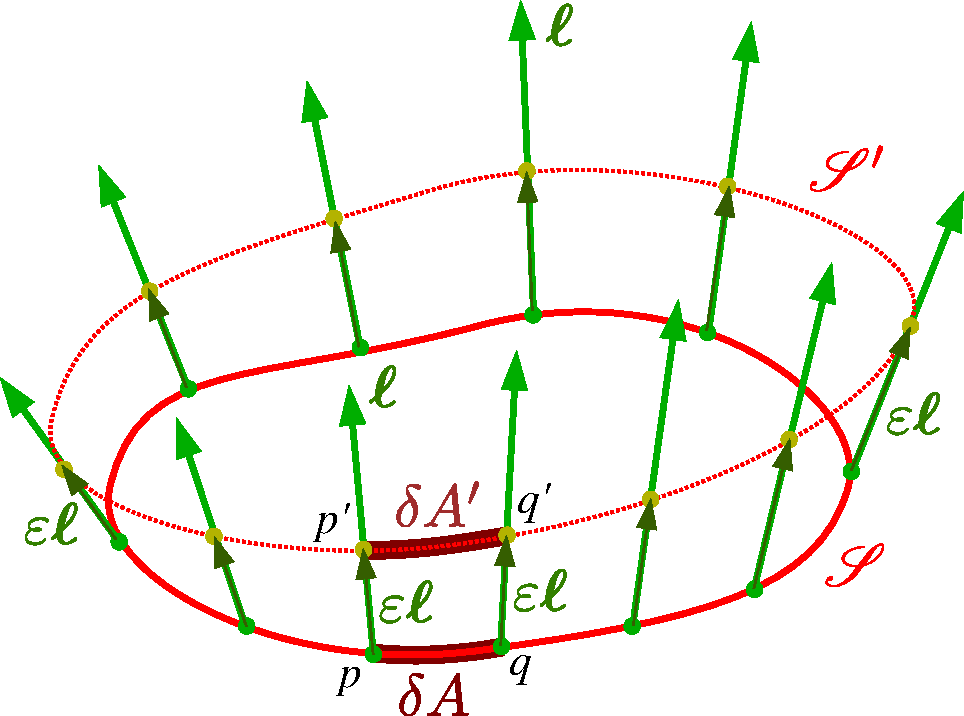
\includegraphics[width=0.6\textwidth]{def_expansion.pdf}}
\caption[]{\label{f:def:expansion} \footnotesize
Lie dragging of the surface $\Sp$ along $\wl$ by the small parameter $\varepsilon$.
$\Sp$ is drawn as a 1-dimensional submanifold, while it is actually a
$(n-2)$-dimensional one, $n$ being the spacetime dimension.}
\end{figure}

\subsection{Expansion along the null normal}

Let us define the expansion of the cross-section $\Sp$ along the vector
field $\wl$ as follows. Given an infinitesimal parameter $\varepsilon\geq 0$, take a point
$p\in \Sp$ and displace it by the infinitesimal vector $\varepsilon \wl$, thereby getting
a nearby point $p_\varepsilon$ (cf. Fig.~\ref{f:def:expansion}).
Since $\wl$ is tangent to $\Hor$ and $p\in\Hor$, we have $p_\varepsilon\in\Hor$.
By repeating this for each point in $\Sp$,
keeping the value of $\varepsilon$ fixed, we define a new codimension-2 surface,
$\Sp_\varepsilon$ say cf. Fig.~\ref{f:def:expansion}). One says that $\Sp_\varepsilon$ is obtained
from $\Sp$ by \defin{Lie dragging along $\wl$ by the parameter $\varepsilon$}\index{Lie!dragging}.
Note that $\Sp_0 = \Sp$.
Since $p_\varepsilon\in\Hor$ for every $p\in\Sp$, we have $\Sp_\varepsilon\subset \Hor$.
Because the null direction $\wl$ is transverse to $\Sp_\varepsilon$ by construction, it
follows that $\Sp_\varepsilon$ is spacelilke (cf. the lemma in Sec.~??).

At each point $p\in\Sp$, the \defin{expansion of $\Sp$ along $\wl$} is defined from the
rate of change $\theta_{(\wl)}$ of the area $\delta A$ of an element of surface $\delta S$ of
$\Sp$ around $p$:
\be \label{e:def:def_expansion}
    \theta_{(\wl)} := \lim_{\varepsilon\rightarrow 0} \frac{1}{\varepsilon}
    \frac{\delta A_\varepsilon - \delta A}{\delta A} .
\ee
In the above formula, $\delta A_\varepsilon$ stands for the area of the
surface element $\delta S_\varepsilon\subset \Sp_\varepsilon$ that is obtained from $\delta S$ by
Lie dragging along $\wl$ by the parameter $\varepsilon$ (cf. Fig.~\ref{f:def:expansion}).
\begin{remark} \label{r:def:expansion_indpt_S}
The reader may wonder why the expansion is not denoted by something like
$\theta_{(\wl)}(\Sp)$, since its definition depends explicitely on
$\Sp$. We shall below that, because $\Hor$ is a null hypersurface, $\theta_{(\wl)}$
is actually independent of the choice of the cross-section $\Sp$.
\end{remark}


For concreteness, let us assume that the element of surface $\delta S \subset\Sp$ is a $(n-2)$-dimensional
parallelogram delimited by some infinitesimal displacement vectors
$\D\w{x}_{(2)},\ldots,\D\w{x}_{(n-1)}$. The area of $\delta S$ is then
\be \label{e:def:A_wepsS_dx}
    \delta A = \wepsS(\D\w{x}_{(2)},\ldots,\D\w{x}_{(n-1)}),
\ee
where $\wepsS$ is the Levi-Civita tensor\index{Levi-Civita!tensor}
associated with the metric $\w{q}$
in $\Sp$ (cf. Sec.~\ref{s:bas:Levi-Civita_tensor} in Appendix~\ref{s:bas}).
Since $\w{q}$ is the metric induced by $\w{g}$ in $\Sp$ and $(\w{n},\w{s})$
is an orthonormal basis of $T_p^\perp \Sp$, $\wepsS$ is actually the
alternating form induced on $\Sp$ by the spacetime Levi-Civita tensor
$\weps$:
\be \label{e:def:epsS_ns}
    \encadre{ \wepsS = \weps(\w{n},\w{s},\ldots) },
\ee
or, in index notation,
\[
    \epsS_{\alpha_1\cdots\alpha_{n-2}} = \eps_{\mu\nu\alpha_1\cdots\alpha_{n-2}} n^\mu s^\nu .
\]
\begin{proof}
To demonstrate (\ref{e:def:epsS_ns}), it sufficies to note that its right-hand side
defines a fully antisymmetric $(n-2)$-linear form on $T_p\Sp$. Since the space
of such forms is 1-dimensional (for $\dim T_p\Sp = n-2$), we have then
necessarily $\wepsS = a \weps$ for some proportionality factor $a$. Since
$\weps(\w{n},\w{s},\D\w{x}_{(2)},\ldots,\D\w{x}_{(n-1)})$ is the volume
of the $n$-parallelepiped construted on the vectors $\w{n},\w{s},\D\w{x}_{(2)},\ldots,\D\w{x}_{(n-1)}$ and $\w{n}$ and $\w{s}$ are unit-length vectors for the metric $\w{g}$,
we have
\[
    \weps(\w{n},\w{s},\D\w{x}_{(2)},\ldots,\D\w{x}_{(n-1)}) = \delta A.
\]
This implies that $a=1$, thereby establishing (\ref{e:def:epsS_ns}).
\end{proof}
An alternative expression of $\wepsS$ is obtained by substituting (\ref{e:def:ns_lk})
for $\w{n}$ and $\w{s}$ in (\ref{e:def:epsS_ns}). Thanks to the multilinearity
and antisymmetry of $\weps$, we get
\be
    \encadre{ \wepsS = \weps(\w{k},\wl,\ldots) } .
\ee

Let us consider in some vicinity of $\Sp$ a coordinate system
\[
    x^\alpha = \left(\varepsilon, u, x^2,\ldots, x^{n-1}\right)
\]
that is adapted to $\Sp$ and $\wl$ in the sense that
\be \label{e:def:l_dsdeps}
    \wl = \der{}{\varepsilon}
\ee
and the points of $\Sp$ are defined by $(\varepsilon,u) = (0,0)$.
Then, from the very definition of the Lie dragging of $\Sp$ along $\wl$, we
have
\be
    \Sp_\varepsilon = \left\{ p\in\M,\quad  (x^0(p), x^1(p)) = (\varepsilon,0)
                        \right\}
\ee
and  $x^a = (x^2,\ldots, x^{n-1})$ can  be viewed as a coordinate system\footnote{
Latin indices from the beginning of the alphabet, $a$, $b$, etc. range from $2$
to $n-1$.} on each surface $\Sp_\varepsilon$.
Let us choose the $n-2$ infinitesimal displacement vectors in (\ref{e:def:A_wepsS_dx})
along the coordinate lines of this system:
\be
    \D x_{(i)}^a = (\underbrace{0,\ldots,0}_{i-2},\D x^i,
                    \underbrace{0,\ldots,0}_{n-1-i}), \qquad
                    2\leq i \leq n-1 .
\ee
Then expression~(\ref{e:def:A_wepsS_dx}) for the area of $\delta S$ becomes
\bea
    \delta A & = & \epsS_{a_1 \cdots a_{n-2}} \, \D x_{(2)}^{a_1} \cdots \D x_{(n-1)}^{a_{n-2}}
                    \nonumber \\
            & = & \epsS_{2\cdots(n-1)} \, \D x^2 \cdots \D x^{n-1} \nonumber \\
     \delta A  & = & \sqrt{q} \, \D x^2 \cdots \D x^{n-1} , \label{e:def:A_sqrt_q}
\eea
where we have used (\ref{e:bas:eps_sqrt_g}) for the components of the
Levi-Civita tensor $\wepsS$, $q$ standing for the determinant of the metric
$\w{q}$ with respect to the coordinates $(x^2,\ldots,x^{n-1})$.
By the very definition of the Lie dragging, the surface element
$\delta S_\varepsilon$ on $\Sp_\varepsilon$
is defined by the same values of the coordinates $(x^2,\ldots, x^{n-1})$
as $\Sp$. In particular, the small coordinate increments $\D x^2$, ..., $\D x^{n-1}$
take the same values as on $\Sp$. Therefore, the area of $\delta S_\varepsilon$
is
\be \label{e:def:A_eps_sqrt_q}
    \delta A_\varepsilon = \sqrt{q(\varepsilon)} \, \D x^2 \cdots \D x^{n-1} ,
\ee
where $q(\varepsilon)$ stands for the determinant of the components of the
metric $\w{q}(\varepsilon)$ induced by $\w{g}$ on $\Sp_\varepsilon$. Since
$\Sp_\varepsilon$ is spacelike (cf. above), $\w{q}(\varepsilon)$ is positive definite, so
that $q(\varepsilon)\geq 0$.

In view of (\ref{e:def:A_sqrt_q})-(\ref{e:def:A_eps_sqrt_q}), the definition (\ref{e:def:def_expansion})
of the expansion of $\Sp$ along $\wl$ can be rewritten as
\[
    \theta_{(\wl)} = \lim_{\varepsilon\rightarrow 0} \frac{1}{\varepsilon}
    \frac{\sqrt{q(\varepsilon)} - \sqrt{q(0)}}{\sqrt{q(0)}} .
\]
We recognize the derivative of the function $\varepsilon \mapsto \ln \sqrt{q(\varepsilon)}=
1/2\, \ln q(\varepsilon)$ at $\varepsilon=0$:
\be \label{e:def:theta_deps_ln_q}
     \theta_{(\wl)} = \frac{1}{2} \frac{\D}{\D\varepsilon}  \ln q .
\ee
Given that $\Sp_\varepsilon$ is deduced from $\Sp$ by a Lie dragging along $\wl$
and $\varepsilon$ is the parameter associated with $\wl$ [cf. Eq.~(\ref{e:def:l_dsdeps})], we may
rewrite this formula as the Lie derivative of $\ln q$ along $\wl$:
\be \label{e:def:theta_Lie_ln_q}
    \theta_{(\wl)} = \frac{1}{2} \Lie{\el} \ln q .
\ee
\begin{example} \label{x:def:light_cone6}
Considering the example of the light cone in Minkowkski spacetime,
it is easy to evaluate $\theta_{(\wl)}$ by means of the spherical coordinates
introduced in Example~\ref{x:def:light_cone5}, since these coordinates are adapted to the
surface $\Sp$, the metric of $\Sp$ being $q_{ab} \D x^a \D x^b = r^2 \D \theta^2
+ r^2\sin^2\theta \D \phi^2$ [cf. Eq.~(\ref{e:def:q_light_cone_spher})].
We have then  $q = \det(q_{ab}) = r^4\sin^2\theta$. Moreover the parameter $\varepsilon$
can be chosen as $\varepsilon = t - t_0$ since $t$ is an (affine) parameter
associated with $\wl$ (cf. Example~\ref{x:def:light_cone3}). Given that
$t=r$ on $\Hor$, we have $\varepsilon = r - t_0$, so that (\ref{e:def:theta_deps_ln_q})
yields
\[
    \theta_{(\wl)} = \frac{1}{2} \frac{\D}{\D r}  \ln q =
         \frac{1}{2} \frac{\D}{\D r} \left( 4 \ln r + 2 \ln\sin\theta \right) ,
\]
i.e.
\[
    \theta_{(\wl)} = \frac{2}{r} .
\]
\end{example}

Using the general law of variation of a derminant, as given by Eq.~(\ref{e:bas:variation_det})
in Appendix~\ref{s:bas}, Eq.~(\ref{e:def:theta_Lie_ln_q}) can be rewritten as
\[
    \theta_{(\wl)} = \frac{1}{2} \, \mathrm{tr} \left(Q^{-1} \times \Lie{\el} Q \right) ,
\]
when $Q$ is the matrix representing the components of $\w{q}$ with respect to the
coordinates $(x^a) = (x^2,\ldots, x^{n-1})$. In index notation, we have
$Q = (q_{ab})$ and $Q^{-1} = (q^{ab})$. Hence
\be \label{e:def:theta_q_ab}
    \theta_{(\wl)} = \frac{1}{2} \, q^{ab} \Liec{\el} q_{ab} .
\ee
We may wonder about the link between the Lie derivative along $\wl$ of the $(n-2)$-metric
$\w{q}$ of the cross-sections $\Sp_\varepsilon$, which appears above, and
the Lie derivative along $\wl$ of the spacetime extension $\w{q}$ defined by
(\ref{e:def:q_g_k_l}). For the sake of clarity, let us denote here the latter
by $\w{\bar q}$. More precisely, we may consider that $\w{\bar q}$ is a
field defined in some neighbourhood of the portion of $\Hor$ sliced by
$\bigcup_{\varepsilon} \Sp_\varepsilon$ via (\ref{e:def:q_g_k_l}), with $\w{k}$
defined at each point $p\in\Sp_\varepsilon$ as the unique null vector of
$T_p^\perp\Sp_\varepsilon$ obeying $\wl\cdot\w{k}=-1$.
Let $\w{u}$ and $\w{v}$ be vector fields on $\Hor$ that are tangent
to the cross-sections $\Sp_\varepsilon$. Applying the bilinear form
$\Lie{\el}\w{\bar q}$ to them and using the Leibniz rule to expand
$\Lie{\el} \left[ \w{\bar q}(\w{u},\w{v}) \right]$ yields
\be \label{e:def:Lie_l_bar_q}
     \Lie{\el} \w{\bar q} \, (\w{u},\w{v}) = \Lie{\el} \left[ \w{\bar q}(\w{u},\w{v}) \right]
        - \w{\bar q}\left(\Lie{\el}\w{u},\w{v}\right)
         - \w{\bar q}\left(\w{u},\Lie{\el}\w{v}\right) .
\ee
Now, since $\w{u}$ and $\w{v}$ are tangent to $\Sp_\varepsilon$, we may
write $\w{\bar q}(\w{u},\w{v}) = \w{q}(\w{u},\w{v})$. Moreover, by the very
definition of a Lie derivative of a vector field (cf. Sec.~\ref{s:bas:Lie}
in Appendix~\ref{s:bas}) and the fact that the cross-sections
$\Sp_\varepsilon$ are Lie-dragged along $\wl$, the vectors
$\Lie{\el}\w{u}$ and $\Lie{\el}\w{v}$ are also tangent to $\Sp_\varepsilon$.
Therefore, we have
\[
    \w{\bar q}\left(\Lie{\el}\w{u},\w{v}\right) = \w{q} \left(\Lie{\el}\w{u},\w{v}\right)
    \quad\mbox{and}\quad
    \w{\bar q}\left(\w{u},\Lie{\el}\w{v}\right) = \w{q}\left(\w{u},\Lie{\el}\w{v}\right)
\]
as well. Thus, we may rewrite (\ref{e:def:Lie_l_bar_q}) as
\[
     \Lie{\el} \w{\bar q} \, (\w{u},\w{v}) = \Lie{\el} \left[ \w{q}(\w{u},\w{v}) \right]
        - \w{q}\left(\Lie{\el}\w{u},\w{v}\right)
         - \w{q}\left(\w{u},\Lie{\el}\w{v}\right) .
\]
The right-hand side being identical to what would be obtained by expressing
$\Lie{\el} \w{q} \, (\w{u},\w{v})$ via the Leibniz rule. Hence we conclude
that
\[
    \Lie{\el} \w{\bar q} \, (\w{u},\w{v}) = \Lie{\el} \w{q} \, (\w{u},\w{v}) .
\]
Since this identity holds for a pair $(\w{u},\w{v})$ of vectors tangent
to $\Sp_\varepsilon$, we may express it for any pair of vectors, i.e. not
necessarily tangent to $\Sp_\varepsilon$ by introducing the orthogonal
projector $\vw{q}$ onto $\Sp_\varepsilon$ [cf. Eq.~(\ref{e:def:q_proj})]:
\[
    \Lie{\el} \w{\bar q} \, (\vw{q}(\w{u}),\vw{q}(\w{v})) =
    \Lie{\el} \w{q} \, (\vw{q}(\w{u}),\vw{q}(\w{v})) .
\]
Using index notation, this is equivalent to
\[
    \Liec{\el} {\bar q}_{\mu\nu} \, {\bar q}^\mu_{\ \, \alpha} {\bar q}^\nu_{\ \, \beta} =
        \Liec{\el} {q}_{ab} \, {\bar q}^a_{\ \, \alpha} {\bar q}^b_{\ \, \beta} .
\]
Taking the trace with respect to $\w{g}$, we get
\[
    \Liec{\el} {\bar q}_{\mu\nu} \, {\bar q}^\mu_{\ \, \sigma} {\bar q}^{\nu\sigma} =
        \Liec{\el} {q}_{ab} \, {\bar q}^a_{\ \, \sigma} {\bar q}^{b\sigma} .
\]
Now, since $\w{\bar q}$ is symmetric and $\vw{q}$ is a projector,
${\bar q}^\mu_{\ \, \sigma} {\bar q}^{\nu\sigma} = {\bar q}^\mu_{\ \, \sigma} {\bar q}^{\sigma\nu}
 = {\bar q}^{\mu\nu}$. Similarly, ${\bar q}^a_{\ \, \sigma} {\bar q}^{b\sigma} = {\bar q}^{ab}$.
Hence
\[
    {\bar q}^{\mu\nu} \Liec{\el} {\bar q}_{\mu\nu} = {\bar q}^{ab}  \Liec{\el} {q}_{ab}
    = q^{ab}  \Liec{\el} {q}_{ab} ,
\]
where the second equality follows from
${\bar q}^{ab}  = q^{ab}$.
Hence we may rewrite (\ref{e:def:theta_q_ab}) as
\be \label{e:def:theta_q_munu}
    \theta_{(\wl)} = \frac{1}{2} \, q^{\mu\nu} \Liec{\el} q_{\mu\nu} .
\ee
Note that we have dropped the bar over $q$, i.e. we revert to previous notation.

Substituting (\ref{e:def:q_g_k_l}) for $q_{\mu\nu}$, and using Leibniz rule, we get
\[
    \theta_{(\wl)} = \frac{1}{2} \, q^{\mu\nu}  \left(
            \Liec{\el} g_{\mu\nu} + \Liec{\el}  \el_\mu \; k_\nu + \el_\mu \, \Liec{\el} k_\nu
           + \Liec{\el} k_\mu \; \el_\nu + k_\mu \, \Liec{\el} \el_\nu \right) .
\]
If we express the Lie derivative $\Liec{\el} g_{\mu\nu}$ in terms of the
covariant derivative $\wnab$ via Eq.~(\ref{e:bas:Lie_der_comp_nab}) of
Appendix~{\ref{s:bas}, we get
\[
    \Liec{\el} g_{\mu\nu} = \el^\sigma \underbrace{\nabla_\sigma g_{\mu\nu}}_{0}
        + \underbrace{g_{\sigma\nu} \nabla_\mu \el^\sigma}_{\nabla_\mu \el_\nu}
        + \underbrace{g_{\mu\sigma} \nabla_\nu \el^\sigma}_{\nabla_\nu \el_\mu}
       = \nabla_\mu \el_\nu + \nabla_\nu \el_\mu .
\]
Moreover, since $\wl$ and $\w{k}$ are orthogonal to $\Sp$, we have
\[
    q^{\mu\nu} \el_\nu = 0 \quad\mbox{and}\quad
    q^{\mu\nu} k_\nu = 0 .
\]
Hence we end up with
\[
    \theta_{(\wl)} = \frac{1}{2} \, q^{\mu\nu}  \left( \nabla_\mu \el_\nu + \nabla_\nu \el_\mu
        \right) ,
\]
i.e. since $q^{\mu\nu}$ is symmetric,
\be
    \encadre{ \theta_{(\wl)} = q^{\mu\nu} \nabla_\mu \el_\nu } .
\ee

We can transform further this relation by expressing $q^{\mu\nu}$ via (\ref{e:def:q_g_k_l}):
\bea
    \theta_{(\wl)} & = & \left( g^{\mu\nu} + \el^\mu k^\nu + k^\mu \el^\nu \right)
        \nabla_\mu \el_\nu  \nonumber \\
        & = & \nabla_\mu \el^\mu + k^\nu \underbrace{\el^\mu  \nabla_\mu \el_\nu }_{\kappa \el_\nu}
            + k^\mu \el^\nu  \nabla_\mu \el_\nu \nonumber \\
        & = & \nabla_\mu \el^\mu + \kappa \underbrace{k^\nu \el_\nu}_{-1}
            + \frac{1}{2} \underbrace{k^\mu \nabla_\mu (\el_\nu \el^\nu)}_{0}
            \nonumber \\
        & = & \nabla_\mu \el^\mu - \kappa , \label{e:def:theta_div_l_index}
\eea
where we have used respectively the properties (\ref{e:def:wl_geod_kappa}),
(\ref{e:def:el_nab_el_zero}) and (\ref{e:def:k_el_minus_one}).
Denoting the divergence of $\wl$ by $\wnab\cdot\wl = \nabla_\mu \el^\mu$, we
have then
\be \label{e:def:theta_div_l}
    \encadre{\theta_{(\wl)} = \wnab\cdot\wl - \kappa } .
\ee
\begin{remark} \label{r:def:theta_div_l}
Contrary to $\theta_{(\wl)}$ or $\kappa$, the quantity $\wnab\cdot\wl$ depends
on the extension of $\wl$ outside $\Hor$ (cf. the discussion in Sec.~\ref{s:def:null_gener}).
For Eq.~(\ref{e:def:theta_div_l}) to hold, we have supposed that $\wl$ remains null
outside $\Hor$, so that $k^\mu\nabla_\mu(\el_\nu \el^\nu)$, which is a
derivative in a direction transverse to $\Hor$, could be set to zero
in the computation leading to (\ref{e:def:theta_div_l_index}).
\end{remark}

\begin{example}  \label{x:def:light_cone7}
For the light cone in Minkowksi space, $\wnab\cdot\wl$ is easily computed by taking the trace of
(\ref{e:def:nab_l_light_cone}) and we have $\kappa=0$ (cf. Example~\ref{x:def:light_cone3}),
so that (\ref{e:def:theta_div_l}) yields
\[
    \theta_{(\wl)} = \frac{2(x^2+y^2+z^2)}{r^3} = \frac{2}{r} .
\]
Hence we recover the result obtained in Example~\ref{x:def:light_cone6}.
\end{example}

We notice that the right-hand side of (\ref{e:def:theta_div_l}) is independent of the
explicit choice of the cross-section $\Sp$: clearly both $\wnab\cdot\wl$
and $\kappa$ depends only on the null normal $\wl$ of $\Hor$. This justifies
the notation $\theta_{(\wl)}$, which does not refer to $\Sp$
(cf. Remark~\ref{r:def:expansion_indpt_S} in page~\pageref{r:def:expansion_indpt_S}).
This can be understood geometrically as follows. Let $p\in\Hor$ be a
point where one would like to evaluate $\theta_{(\wl)}$. Let $\Sp$ and $\Sp'$
be two distinct cross-sections of $\Hor$ going through $p$
(cf. Fig.~??). Let $q$ be a point of $\Sp$ infinitely close to $p$ and let $q'$
be the point of $\Sp'$ located on the same null generator as $q$,
i.e. $\vec{qq'} = \varepsilon \wl$, with $\varepsilon$ infinitely small.
Let $\D\w{x}$ (resp. $\D\w{x'}$) be the infinitesimal vector connecting
$p$ to $q$ (resp. $p$ to $q'$). We have then
\[
\D\w{x'} = \D\w{x} + \varepsilon \wl ,
\]
the scalar square of which is
\[
    \D\w{x'}\cdot\D\w{x'} =\D\w{x}\cdot\D\w{x}
            + 2 \varepsilon \underbrace{\D\w{x}\cdot \wl}_{0}
            + \underbrace{\wl\cdot \wl}_{0},
\]
where we have the fact that $\wl$ is normal to any vector tangent to $\Sp$,
such as $\D\w{x}$ and $\wl$ is null. Hence
\[
    \D\w{x'}\cdot\D\w{x'} = \D\w{x}\cdot\D\w{x} .
\]
In other words, the lengths of all segments from $p$ do not depend
on the cross-section in which they are taken, provided their second end
lies on the same null generator of $\Hor$. It follows that all infinitesimal surfaces
$\delta S$ around $p$ that are enclosed in tube made of null generators have the same
area $\delta A$. Hence the expansion $\theta_{(\wl)}$ at $p$
does not depend on the choice of $\delta S$, i.e. of the cross-section
$\Sp$ through $p$.
We conclude that
\begin{quote}
The expansion $\theta_{(\wl)}$ depends only on the choice of the null
normal $\wl$ on the null hypersurface $\Hor$.
\end{quote}
For this reason, from now on, we shall call $\theta_{(\wl)}$
the \defin{expansion of the null hypersurface $\Hor$ along $\wl$}\index{expansion!of a null hypersurface}.

The dependency of the expansion on $\wl$ is given by the following
behaviour under a rescaling of $\wl$:
\be \label{e:def:rescale_lambda}
   \wl' = \alpha \wl \ \Longrightarrow \ \theta_{(\wl')} = \alpha \theta_{(\wl)} ,
\ee
where $\alpha$ is any positive scalar field on $\Hor$. This follows immediately
from the expression (\ref{e:def:theta_Lie_ln_q}) of $\theta_{(\wl)}$, given
that the metric $\w{q}$ is independent of $\wl$ and
$\w{\Liesymbol}_{\alpha\wl}\,\ln q = \alpha \Lie{\wl}\ln q$.
\begin{remark}
The reader may check that the rescaling laws (\ref{e:def:rescale_kappa})
and (\ref{e:def:rescale_lambda}) for respectively $\kappa$ and $\theta_{(\wl)}$
are compatible with the expression (\ref{e:def:theta_div_l}) of $\theta_{(\wl)}$,
given that $\wnab\cdot \wl' = \alpha\wnab\cdot\wl + \wnab_{\wl} \alpha$.
\end{remark}

Let us gather all the expressions of the expansion $\theta_{(\wl)}$ obtained
so far:
\be \label{e:def:theta_l_all}
    \encadre{ \theta_{(\wl)} = \lim_{\varepsilon\rightarrow 0} \frac{1}{\varepsilon}
    \frac{\delta A_\varepsilon - \delta A}{\delta A}
        = \frac{1}{2} \Lie{\el} \ln q
        = \frac{1}{2} \, q^{\mu\nu} \Liec{\el} q_{\mu\nu}
        = q^{\mu\nu} \nabla_\mu \el_\nu
        = \wnab\cdot\wl - \kappa } ,
\ee
with the reminder that the last expression is valid insofar as the vector field $\wl$ is
null in some entire open neighborhood of $\Hor$ (and not only on $\Hor$), as
stressed in Remark~\ref{r:def:theta_div_l}.

\subsection{Deformation rate and shear tensor}

Let us consider a cross-section $\Sp$ of the null hypersurface $\Hor$.
The \defin{deformation rate}\index{deformation rate} $\w{\Theta}$ of $\Sp$ is defined from the Lie
derivative of the induced metric $\w{q}$ of $\Sp$ along $\wl$ as
\be \label{e:def:Theta}
    \w{\Theta} := \frac{1}{2} \vw{q}^* \Lie{\el} \w{q} ,
\ee
where $\vw{q}^*$ stands for the action of the orthogonal projector $\vw{q}$
onto $\Sp$ on the bilinear form $\Lie{\el} \w{q}$.
This action extends $\Lie{\el} \w{q}$, which is defined a priori on
vectors of $T_p\Sp$ to all vectors of $T_p\M$, for any $p\in\Sp$, via
\be
    \forall (\w{u},\w{v}) \in T_p\M \times T_p\M, \quad
         \vw{q}^* \Lie{\el} \w{q}\,  (\w{u}, \w{v}) =
         \Lie{\el} \w{q} \left( \vw{q}(\w{u}), \vw{q}(\w{v}) \right) .
\ee
Accordingly, the index-notation version of (\ref{e:def:Theta}) is
\be \label{e:def:Theta_index}
    \Theta_{\alpha\beta} = \frac{1}{2} q^\mu_{\ \, \alpha} q^\nu_{\ \, \beta}
            \Liec{\el} q_{\mu\nu} .
\ee
Since $\w{q}$ is symmetric, it is clear from the above definition that
$\w{\Theta}$ is a symmetric bilinear form.

Expressing the Lie derivative in terms of the covariant derivative
$\wnab$ via Eq.~(\ref{e:bas:Lie_der_comp_nab}) of Appendix~{\ref{s:bas}
and using expression (\ref{e:def:q_g_k_l}) of $\w{q}$, we get
\bea
    \Theta_{\alpha\beta} & = & \frac{1}{2} q^\mu_{\ \, \alpha} q^\nu_{\ \, \beta}
        \left( \el^\sigma \nabla_\sigma q_{\mu\nu}
            + q_{\sigma\nu}\nabla_\mu \el^\sigma
            + q_{\mu\sigma}\nabla_\nu \el^\sigma \right) \nonumber \\
            & = & \frac{1}{2} q^\mu_{\ \, \alpha} q^\nu_{\ \, \beta} \Big[
                l^\sigma \left( \nabla_\sigma \el_\mu k_\nu
                    + \el_\mu \nabla_\sigma k_\nu +  \nabla_\sigma k_\mu \el_\nu
                    + k_\mu \nabla_\sigma \el_\nu \right) \nonumber \\
            & & \qquad\qquad + \nabla_\mu \el_\nu + k_\nu \underbrace{\el_\sigma \nabla_\mu \el^\sigma}_{0}
                + k_\sigma \el_\nu \nabla_\mu \el^\sigma  + \nabla_\nu \el_\mu + \el_\mu k_\sigma \nabla_\nu \el^\sigma
                + k_\mu \underbrace{\el_\sigma \nabla_\nu \el^\sigma}_{0}
                                    \Big] . \nonumber
\eea
Since $q^\mu_{\ \, \alpha} \el_\mu = 0$ and $q^\mu_{\ \, \alpha} k_\mu = 0$,
the above expression simplies to
\be
    \Theta_{\alpha\beta}  = q^\mu_{\ \, \alpha} q^\nu_{\ \, \beta} \nabla_\mu \el_\nu .
\ee
Let us substitute (\ref{e:def:q_proj}) for the projector $\vw{q}$:
\[
    \Theta_{\alpha\beta}  = \left(\delta^\mu_{\ \, \alpha}
        + \el^\mu k_\alpha + k^\mu \el_\alpha \right)
        \left(\delta^\nu_{\ \, \beta}
        + \el^\nu k_\beta + k^\nu \el_\beta \right) \nabla_\mu \el_\nu .
\]
Expanding and simplifying (in particular via $\el^\nu \nabla_\mu \el_\nu = 0$)
yields
\be \label{e:def:nab_l_Theta}
   \encadre{ \nabla_\alpha \el_\beta = \Theta_{\alpha\beta}
        + \omega_\alpha \el_\beta - \el_\alpha k^\mu \nabla_\mu \el_\beta },
\ee
with
\be \label{e:def:def_omega}
    \omega_\alpha := - k^\mu \nabla_\alpha \el_\mu - k^\mu k^\nu \nabla_\mu \el_\nu \, \el_\alpha .
\ee
\begin{remark}
The 1-form $\w{\omega}$ is sometimes called the \defin{rotation 1-form} of
the cross-section $\Sp$; see Ref.~\cite{GourgJ06} for details.
\end{remark}

By comparing (\ref{e:def:theta_q_munu}) and (\ref{e:def:Theta_index}), we
notice that the trace of $\w{\Theta}$ is nothing but the expansion
$\theta_{(\wl)}$:
\be
    \theta_{(\wl)} = g^{\mu\nu} \Theta_{\mu\nu} = q^{\mu\nu} \Theta_{\mu\nu} = \Theta^\mu_{\ \, \mu} .
\ee
The trace-free part of $\w{\Theta}$ is called the \defin{shear tensor}\index{shear!tensor}
of $\Sp$:
\be \label{e:def:def_shear}
    \w{\sigma} := \w{\Theta} - \frac{1}{n-2} \theta_{(\wl)} \, \w{q} ,
\ee
or, in index notation:
\be
    \sigma_{\alpha\beta} = \Theta_{\alpha\beta} - \frac{1}{n-2} \theta_{(\wl)} \, q_{\alpha\beta} .
\ee
Note that the $1/(n-2)$ factor arises from the trace of $\w{q}$, which is $n-2$,
as easily seen from (\ref{e:def:q_g_k_l}):
\be
    q^\mu_{\ \, \mu} = \underbrace{\delta^\mu_{\ \, \mu}}_{n}
                    + 2 \underbrace{\el^\mu k^\mu}_{-1} = n - 2 .
\ee
By construction, we have thus
\be
    \sigma^\mu_{\ \, \mu} = g^{\mu\nu} \sigma_{\mu\nu} = q^{\mu\nu} \sigma_{\mu\nu} = 0 .
\ee
Note that $\w{\Theta}$ and $\w{\sigma}$ are tensor fields tangent to $\Sp$, in the sense
that
\be \label{e:def:Theta_sigma_tangent}
    \forall \w{v}\in T_p^\perp \Sp, \quad \w{\Theta}(\w{v}, .) = \w{\sigma}(\w{v}, .) = 0 ,
\ee
with the important special cases $\w{v} = \wl$ and $\w{v} = \w{k}$.

\begin{remark}
Contrary to $\theta_{(\wl)}$ which depends only on $\wl$, the tensor fields
$\w{\Theta}$ and $\w{\sigma}$ depend on the specific choice of the cross-section $\Sp$,
in addition to $\wl$.
\end{remark}

\begin{example} \label{x:def:light_cone8}
Let us consider the light cone in Minkowski spacetime (cf. Example~\ref{x:def:light_cone6}).
Since the coordinates $(t,\theta,\phi)$
are adapted to the vector field $\wl$ (i.e. the $\theta$ and $\phi$ are constant
along the field lines of $\wl$ on $\Hor$ and $\wl = \partial/\partial t$ in these
coordinates, in other words, $\el^\alpha=(1,0,0)$), we have (cf. formula~(\ref{e:bas:Lie_adapted})
in Appendix~\ref{s:bas})
\[
    \Liec{\el} q_{ab} = \der{}{t} q_{ab} = \der{}{r} q_{ab} ,
\]
where the second equality follows from $t=r$ on $\Hor$. Given that
$q_{ab} = \mathrm{diag}(r^2, r^2\sin^2\theta)$
[cf. Eq.~(\ref{e:def:q_light_cone_spher})], we obtain
\[
    \Liec{\el} q_{ab} = \left( \begin{array}{cc}
        2 r & 0  \\
        0 & 2 r \sin^2\theta
        \end{array} \right)
        = \frac{2}{r} \, q_{ab} .
\]
Hence (\ref{e:def:Theta}) yields
\[
    \w{\Theta} = \frac{1}{r} \, \w{q} .
\]
Taking the trace, we get immediately $\theta_{(\wl)} = 2/r$, i.e. we recover
the result of Examples~\ref{x:def:light_cone6} and \ref{x:def:light_cone7}.
From (\ref{e:def:def_shear}), we get a vanishing shear:
\[
    \w{\sigma} = 0 .
\]
\end{example}

\subsection{Null Raychaudhuri equation}

Let us derive an evolution equation for the expansion $\theta_{(\wl)}$.
The starting point is the Ricci identity [Eq.~(\ref{e:bas:Ricci_ident}) in Appendix~\ref{s:bas}]
applied to $\wl$:
\[
   \left(\nabla_\alpha\nabla_\beta
        - \nabla_\beta\nabla_\alpha\right) \el^\gamma
        = R^\gamma_{\ \  \mu \alpha\beta} \, \el^\mu ,
\]
where $R^\gamma_{\ \  \mu \alpha\beta}$ is the Riemann tensor of the metric
$\w{g}$.
Taking the trace on the indices $(\alpha,\gamma)$ and relabeling $\beta\rightarrow\alpha$ yields
\[
    \nabla_\mu \nabla_\alpha \el^\mu - \nabla_\alpha \nabla_\mu \el^\mu =
        R_{\mu\alpha} \el^\mu ,
\]
where $R_{\mu\alpha} = R^\sigma_{\ \  \mu \sigma\alpha}$ is
the Ricci tensor of $\w{g}$.
Substituting Eq.~(\ref{e:def:nab_l_Theta}) for $\nabla_\alpha \el^\mu$ and $\theta_{(\wl)} + \kappa$ for $\nabla_\mu \el^\mu = \wnab\cdot\wl$ [cf. Eq.~(\ref{e:def:theta_div_l})] yields
\[
    \nabla_\mu \left( \Theta_\alpha^{\ \, \mu} + \omega_\alpha \el^\mu - \el_\alpha
        k^\nu \nabla_\nu \el^\mu \right) - \nabla_\alpha \left( \theta_{(\wl)} + \kappa \right) =
        R_{\mu\alpha} \el^\mu .
\]
Expanding the left-hand side and using again Eqs.~(\ref{e:def:theta_div_l}) and
(\ref{e:def:nab_l_Theta}) leads to
\bea
    \nabla_\mu \Theta^\mu_{\ \, \alpha} + \el^\mu \nabla_\mu \omega_\alpha
       - \nabla_\alpha \left( \theta_{(\wl)} + \kappa \right)
        + \left( \theta_{(\wl)} + \kappa \right) \omega_\alpha
        - \Theta_{\alpha\mu} k^\nu \nabla_\nu \el^\mu & & \nonumber \\
    - \left( \omega_\mu k^\nu \nabla_\nu \el^\mu
    + \nabla_\mu k^\nu \nabla_\nu \el^\mu + k^\nu \nabla_\mu \nabla_\nu \el^\mu \right)
        \el_\alpha & = & R_{\mu\alpha} \el^\mu . \label{e:def:contract_Ricci_ident}
\eea
The above relation is a 1-form identity. Applying it to the vector field $\wl$
(i.e. contracting with $\el^\alpha$), we get, since $\el_\nu \el^\nu =0$,
\be \label{e:def:Raychaud_step1}
    \el^\nu \nabla_\mu \Theta^\mu_{\ \, \nu} + \el^\nu \el^\mu \nabla_\mu \omega_\nu
        - \el^\mu \nabla_\mu \left( \theta_{(\wl)} + \kappa \right)
        + \left( \theta_{(\wl)} + \kappa \right) \omega_\mu \el^\mu
        = R_{\mu\nu} \el^\mu \el^\nu .
\ee
Now, using $\Theta^\mu_{\ \, \nu}  \el^\nu = 0$ [Eq.~(\ref{e:def:Theta_sigma_tangent})]
and Eq.~(\ref{e:def:nab_l_Theta}), we can write
\bea
    \el^\nu \nabla_\mu \Theta^\mu_{\ \, \nu} & = & \nabla_\mu
    ( \underbrace{\Theta^\mu_{\ \, \nu} \el^\nu}_{0} )
    - \Theta^\mu_{\ \, \nu} \nabla_\mu \el^\nu = - \Theta^{\mu\nu} \nabla_\mu \el_\nu
    = - \Theta^{\mu\nu}  \left( \Theta_{\mu\nu} + \omega_\mu \el_\nu
        - \el_\mu k^\sigma \nabla_\sigma \el_\nu \right) \nonumber \\
    & = & - \Theta^{\mu\nu}  \Theta_{\mu\nu} . \nonumber
\eea
On the other side,
\[
    \el^\nu \el^\mu \nabla_\mu \omega_\nu = \el^\mu \nabla_\mu (\omega_\nu \el^\nu )
        - \omega_\nu \underbrace{\el^\mu \nabla_\mu \el^\nu}_{\kappa \el^\nu}
        = \el^\mu \nabla_\mu (\omega_\nu \el^\nu ) - \kappa \omega_\nu \el^\nu ,
\]
Accordingly Eq.~(\ref{e:def:Raychaud_step1}) becomes
\[
    - \Theta^{\mu\nu}  \Theta_{\mu\nu}  + \el^\mu \nabla_\mu (\omega_\nu \el^\nu )
        - \el^\mu \nabla_\mu \left( \theta_{(\wl)} + \kappa \right)
        + \theta_{(\wl)} \omega_\mu \el^\mu
        = R_{\mu\nu} \el^\mu \el^\nu .
\]
The term $\omega_\mu \el^\mu$, which appears twice in this equation, takes
a simple form:
\be
    \omega_\mu \el^\mu = \kappa .
\ee
Indeed, from the definition~(\ref{e:def:def_omega}) of the 1-form $\w{\omega}$,
\be \label{e:def:omega_l_kappa}
    \omega_\mu \el^\mu = - k^\nu \underbrace{\el^\mu \nabla_\mu \el_\nu}_{\kappa \el_\nu}
        - k^\rho k^\sigma \nabla_\rho \el_\sigma \, \underbrace{\el_\mu \el^\mu}_{0}
         = - \kappa \underbrace{k^\nu \el_\nu}_{-1} = \kappa .
\ee
Therefore the two derivatives $\el^\mu \nabla_\mu (\omega_\nu \el^\nu )$ and $-\el^\mu \nabla_\mu \kappa$
cancel out and one is left with
\be \label{e:def:Raychaud_step2}
   - \Theta^{\mu\nu}  \Theta_{\mu\nu} - \el^\mu \nabla_\mu \theta_{(\wl)}
    + \kappa \theta_{(\wl)} = R_{\mu\nu} \el^\mu \el^\nu .
\ee
The first term in the left-hand side can be re-expressed by the decomposition
(\ref{e:def:def_shear}) of
$\w{\Theta}$ in terms of the shear tensor and the trace term:
\bea
    \Theta_{\mu\nu} \Theta^{\mu\nu} & = & \left( \sigma_{\mu\nu}
        + \frac{1}{n-2} \, \theta_{(\wl)} q_{\mu\nu} \right)
        \left( \sigma^{\mu\nu}
        + \frac{1}{n-2} \, \theta_{(\wl)} q^{\mu\nu} \right) \nonumber \\
        & = &
     \sigma_{\mu\nu} \sigma^{\mu\nu} + \frac{2}{n-2} \, \theta_{(\wl)}
    \underbrace{q^{\mu\nu} \sigma_{\mu\nu}}_{0}
        + \frac{1}{(n-2)^2}\,  \theta_{(\wl)}^2 \underbrace{q_{\mu\nu} q^{\mu\nu}}_{n-2} \nonumber \\
    & = & \sigma_{\mu\nu} \sigma^{\mu\nu} + \frac{1}{n-2} \, \theta_{(\wl)}^2 , \nonumber \\
    & = & \sigma_{ab} \sigma^{ab} + \frac{1}{n-2} \, \theta_{(\wl)}^2 . \nonumber
\eea
Hence Eq.~(\ref{e:def:Raychaud_step2}) can be rewitten as
\be
    \encadre{ \wnab_{\el}\,  \theta_{(\wl)} = \kappa \theta_{(\wl)}
        - \frac{1}{n-2} \, \theta_{(\wl)}^2 - \sigma_{ab} \sigma^{ab}
        - \w{R}(\wl, \wl) }.
\ee
Since $\wl$ is future-directed, this is an evolution equation for
$\theta_{(\wl)}$. It is known as the
\defin{null Raychaudhuri equation}\index{null!Raychaudhuri equation}\index{Raychaudhuri!null --  equation}.

If the spacetime $(\M,\w{g})$ is ruled by general relativity, i.e. if
$\w{g}$ obeys Einstein equation (\ref{e:bas:Einstein_eq_n}), we may express
the term involving the Ricci tensor in terms of the total energy-momentum tensor
$\w{T}$:
\[
  \w{R}(\wl, \wl)  = \frac{2}{n-2}\,\Lambda\,  \underbrace{\w{g}(\wl, \wl)}_{0}
    + 8\pi \big[ \w{T}(\wl, \wl) - \frac{1}{n-2}\,  T \, \underbrace{\w{g}(\wl, \wl)}_{0} \big]
    = 8\pi \w{T}(\wl, \wl) .
\]
The null Raychaudhuri equation becomes then
\be \label{e:def:null_Raychaud}
    \encadre{ \wnab_{\el}\,  \theta_{(\wl)} = \kappa \theta_{(\wl)}
        - \frac{1}{n-2} \, \theta_{(\wl)}^2 - \sigma_{ab} \sigma^{ab}
        - 8\pi \w{T}(\wl, \wl) }.
\ee

\begin{remark}
Since $\theta_{(\wl)}$ is a scalar field on $\Hor$, $\wnab_{\el}\,  \theta_{(\wl)}$
can be replaced by the Lie derivative $\Lie{\wl} \theta_{(\wl)}$ in the left-hand side of the Raychaudhuri
equation.
\end{remark}

\begin{example}
Let us check the null Raychaudhuri equation on the light cone in Minkowski
spacetime. From Example~\ref{x:def:light_cone3}, we have $\kappa=0$, while
from Example~\ref{x:def:light_cone8}, we have $\w{\sigma}=0$,
hence $\sigma_{ab} \sigma^{ab}=0$. Moreover, the Ricci tensor of Minkowski
spacetime vanishes identically. The null Raychaudhuri equation reduces
then to
\[
    \wnab_{\el}\,  \theta_{(\wl)} =  - \frac{1}{2} \, \theta_{(\wl)}^2 ,
\]
where we have set $n=4$. Now, from Example~\ref{x:def:light_cone6}, we
have $\theta_{(\wl)} = 2/r$. Since, in the present case
$\wnab_{\el}\,  \theta_{(\wl)}  = \Lie{\el} \,  \theta_{(\wl)}  = \dert{\theta_{(\wl)}}{r} =
- 2/r^2$, we conclude that the null Raychaudhuri equation is satisfied (as
it should!).
\end{example}

%%%%%%%%%%%%%%%%%%%%%%%%%%%%%%%%%%%%%%%%%%%%%%%%%%%%%%%%%%%%%%%%%%%%%%%%%%%%%%%

\section{Non-expanding horizons}

\subsection{Motivation and definition}

Having discussed in depth the geometry of null hypersurfaces, and in particular
their expansion, let us make an attempt to distinguish a black hole event
horizon from, let us say, a future light cone.
To get the localized behaviour mentionned in the black hole naive definition
of Sec.~\ref{s:def:first_defin}, we could demand that the area of the
spacelike cross-sections remains constant, in other words that
the expansion along the null normal vanishes. Hence the definition:\\
A \defin{non-expanding horizon} is a null hypersurface $\Hor$ having the
topology (\ref{e:def:H_topology}):
\be
    \Hor \simeq \R \times \mathbb{S}^{n-2}
\ee
and such that the expansion of $\Hor$ along any null normal $\wl$ vanishes
identically:
\be
    \theta_{(\wl)} = 0 .
\ee
Note that, given the scaling law (\ref{e:def:rescale_lambda}),
if $\theta_{(\wl)} = 0$ for some normal $\wl$, then  $\theta_{(\wl')} = 0$
for any other normal $\wl'$. Hence the definition of a non-expanding horizon
does not depend on the choice of the null normal.

As we shall discuss in detail in Chap.~??, this definition captures only
the event horizon of black holes in equilibrium.

\subsection{Trapped surfaces}

If there is a natural concept of \emph{outer}/\emph{inner} for $\Hor$, for
instance the outer region being the one that contains an asymptotically flat end,
and if the transverse null normals $\w{k}$ point to the inner region, then
the property $\theta_{(\wl)}=0$ means that any cross-section $\Sp$ of the
non-expanding horizon $\Hor$ is a
\defin{marginally outer trapped surface}\index{marginally!outer trapped surface}\index{trapped!surface!marginally outer --}
(often abriged as \defin{MOTS}\index{MOTS}). This definition is due to
Hawking \cite{Hawki73}, an
\defin{outer trapped surface}\index{outer!trapped surface}\index{trapped!surface!outer --}
would be one for which $\theta_{(\wl)}\leq 0$.

This definition is related to, but distinct from, the definition of a
marginally trapped surface by Penrose \cite{Penro65}: a $(n-2)$-dimensional
submanifold $\Sp$ of $\M$ is a \defin{trapped surface}\index{trapped!surface}
 iff (i) $\Sp$ is
closed (i.e. compact without boundary), (ii) $\Sp$ is spacelike and (iii)
the two systems of null geodesics emerging orthogonally from $\Sp$ converge
locally at $\Sp$, i.e. they have negative expansions:
\be
    \theta_{(\wl)} < 0 \quad\mbox{and}\quad \theta_{(\w{k})} < 0 ,
\ee
where the expansion along $\w{k}$ is defined in the same way as that along
$\wl$ [cf. Eq.~(\ref{e:def:theta_l_all})]:
\be
    \theta_{(\w{k})} := \lim_{\varepsilon\rightarrow 0} \frac{1}{\varepsilon}
    \frac{\delta A^{(\w{k})}_\varepsilon - \delta A}{\delta A}
        = \frac{1}{2} \Lie{\w{k}} \ln q
        = \frac{1}{2} \, q^{\mu\nu} \Liec{k} q_{\mu\nu}
        = q^{\mu\nu} \nabla_\mu k_\nu ,
\ee
$\delta A^{(\w{k})}_\varepsilon$ begin the area of the surface element
that is deduced from the surface element of area $\delta A$ on $\Sp$ by the
Lie dragging along $\w{k}$ by a parameter $\varepsilon$.
The limit case $\theta_{(\wl)} = 0$ and $\theta_{(\w{k})}<0$ correspond
to the so-called \defin{marginally trapped surface}\index{marginally!trapped!surface}.

In a flat spacetime (Minkowksi), given any spacelike surface,
one has $\theta_{(\wl)} > 0$ and $\theta_{(\w{k})} < 0$ (cf. Fig.~??), so there
is no trapped surface.

Cross-sections of a non-expanding horizon are usually marginally trapped surfaces
(cf. example~??).
However there exist some pathological situations for
which $\theta_{(\w{k})} > 0$ at some points of $\Sp$ \cite{GerocH82}.

\subsection{Vanishing of the deformation rate tensor} \label{s:def:NEH_Theta_zero}

If $\Hor$ is a non-expanding horizon, we may set $\theta_{(\wl)}=0$
in the null Raychaudhuri equation (\ref{e:def:null_Raychaud});it reduces then
to
\be \label{e:def:null_Raychaud_theta_zero}
    \sigma_{ab} \sigma^{ab} + 8\pi \w{T}(\wl, \wl) = 0 .
\ee
The first term is always non-negative:
\be \label{e:def:sigma_square}
    \sigma_{ab} \sigma^{ab} \geq 0 .
\ee
\begin{proof}
Since $\sigma$ is symmetric, it can be diagonalized
in an orthonormal basis of $\w{q}$: $\sigma_{ab} = \mathrm{diag}(s_1,\ldots, s_{n-2})$.
Moreover, $\w{q}$ being a Riemannian metric, we have, in the same basis, $q^{ab} = \mathrm{diag}(1,\ldots,1)$. Since $\sigma^{ab} = q^{am} q^{bn} \sigma_{mn}$, we conclude that
\be \label{e:def:sigma_square_si}
  \sigma_{ab} \sigma^{ab} = s_1^2 + \cdots + s_{n-2}^2 \geq 0 .
\ee
\end{proof}

Regarding the second term in (\ref{e:def:null_Raychaud_theta_zero}), it
is quite natural to assume that matter and non-gravitational fields,
represented by the total energy-momentum tensor $\w{T}$, obey the
\defin{null energy condition}\index{null!energy condition}\index{energy!condition!null --},
namely that
\be \label{e:def:null_energy_cond}
    \w{T}(\wl, \wl) \geq 0 \quad \mbox{for any null vector $\wl$}.
\ee
This condition is pretty weak and is satisfied by
\begin{itemize}
\item vacuum: $\w{T}=0$;
\item any ``reasonable'' matter model, such as a perfect fluid with a
proper energy density $\varepsilon$ and pressure $p$ satisfying
$\varepsilon+p\geq 0$;
\item any electromagnetic field;
\item any real or complex scalar field;
\item ``dark energy'' modeled by $\w{T} = -\frac{\Lambda}{8\pi}\, \w{g}$.
\end{itemize}
Note also that the null energy condition is implied by the
so-called \defin{weak energy condition}\index{weak!energy condition}\index{energy!condition!weak --},
which states that
\be
    \w{T}(\w{u}, \w{u}) \geq 0 \quad \mbox{for any timelike vector $\w{u}$}.
\ee
The null energy condition follows from the
weak energy condition by continuity.
Selecting for $\w{u}$ the 4-velocity of an observer, we see that
the weak energy condition has a simple physical interpretation: the energy
density as measured by any observer is non-negative.

Given (\ref{e:def:sigma_square}) and (\ref{e:def:null_energy_cond}),
Eq.~(\ref{e:def:null_Raychaud_theta_zero})  implies both
\be
    \sigma_{ab} \sigma^{ab}  = 0
\ee
and
\be \label{e:def:T_l_l_zero}
    \w{T}(\wl, \wl) = 0 .
\ee
The identity $\sigma_{ab} \sigma^{ab} = 0$ is possible only if each of
the $s_i$'s in (\ref{e:def:sigma_square_si}) is zero. Hence we have necessarily
\be
    \w{\sigma} = 0 .
\ee
Given $\theta_{(\wl)}=0$, this implies that the full deformation rate tensor
vanishes identically [cf. Eq.~(\ref{e:def:def_shear})]:
\be
    \w{\Theta} = 0 .
\ee
In view of (\ref{e:def:Theta}), this is equivalent to
\be \label{e:def:Lie_el_q_zero}
     \vw{q}^* \Lie{\el} \w{q} = 0 .
\ee
We conclude that, provided that the null energy condition holds,
the whole metric, and not only the area element
$\wepsS$ (as a mere $\theta_{(\wl)}=0$ would suggest), of any cross-section
of a non-expanding horizon is invariant along the null generators.

\subsection{Going further}

See Refs~\cite{GourgJ06,Jaram13,GourgJ08}.


%%%%%%%%%%%%%%%%%%%%%%%%%%%%%%%%%%%%%%%%%%%%%%%%%%%%%%%%%%%%%%%%%%%%%%%%%%%%%%%

\section{Killing horizons}

\subsection{Definition}

A special kind of non-expanding horizons, which is central for the theory of
stationary black holes, is that of Killing horizons. These objects have
been defined by Carter in 1969 \cite{Carte69} as follows: a
\defin{Killing horizon}\index{Killing!horizon}\index{horizon!Killing --} is
a null hypersurface $\Hor$ whose generating null vector $\wl$ can be normalized
so as to coincide with a Killing vector field of $(\M,\w{g})$.

Thus a Killing horizon requires that the spacetime $(\M,\w{g})$ has some symmetry
(usually stationarity), being invariant under the action of a 1-parameter group.
Let us recall that a \defin{Killing vector field}\index{Killing!vector field}
$\w{\xi}$ is a generator of the symmetry group. It can be defined as a vector
field along which the metric tensor is invariant, i.e.
\be \label{e:def:Lie_xi_g}
    \Lie{\xi} \w{g} = 0 .
\ee
Expressing the Lie derivative via Eq.~(\ref{e:bas:Lie_der_comp_nab}) of Appendix~\ref{s:bas},
we see that the above equation is equivalent to the so-called
\defin{Killing equation}\index{Killing!equation}:
\be
    \nabla_\alpha \xi_\beta + \nabla_\beta \xi_\alpha = 0 .
\ee

We shall see in Sec.~?? that in a stationary spacetime, a black hole
event horizon must be a Killing horizon.

\subsection{Killing horizons as non-expanding horizons}

If $\Hor$ is a Killing horizon, then the null normal $\wl$ obeys $\wl \equalH \w{\xi}$,
so that (\ref{e:def:Lie_xi_g}) implies:
\[
    \Lie{\el} \w{g} \equalH 0 .
\]
Let $\Sp$ be a cross-section of $\Hor$; since $\w{q}$ is the metric induced by $\w{g}$
on $\Sp$, we deduce immediately that
\[
    \Lie{\el} \w{q} = 0 .
\]
From the definition (\ref{e:def:Theta})], it follows that the expansion rate
tensor of $\Sp$ vanishes identically:
\[
    \w{\Theta} = 0 .
\]
In particular we have
\[
    \theta_{(\wl)} = 0 .
\]
We conclude that any Killing horizon is a non-expanding horizon.

\subsection{The zeroth law of black hole mechanics}

Let us show that, on a Killing horizon, the non-affinity coefficient $\kappa$
of the null normal $\wl$ coinciding with a Killing vector is constant.

First of all, since $\wl$ is a symmetry generator on $\Hor$, we have
\be
    \Lie{\el} \kappa = 0 ,
\ee
which means that $\kappa$ is constant along the field lines of $\wl$ (i.e. the
null generators of $\Hor$). It could however vary from a field line to another
one. To show that this is not the case, let us consider a cross-section
$\Sp$ of $\Hor$ and project the contracted Ricci identity (\ref{e:def:contract_Ricci_ident})
onto it:
\[
    \nabla_\mu \Theta^\mu_{\ \, \nu} q^\nu_{\ \, \alpha} + \el^\mu \nabla_\mu \omega_\nu q^\nu_{\ \, \alpha}
       - \nabla_\nu \left( \theta_{(\wl)} + \kappa \right) q^\nu_{\ \, \alpha}
        + \left( \theta_{(\wl)} + \kappa \right) \omega_\nu q^\nu_{\ \, \alpha}
        - \Theta_{\alpha\mu} k^\nu \nabla_\nu \el^\mu \nonumber \\
     = R_{\mu\nu} \el^\mu q^\nu_{\ \, \alpha}, \nonumber
\]
where we have used $\Theta_{\nu\mu}  q^\nu_{\ \, \alpha} = \Theta_{\alpha\mu}$
and $\el_\nu q^\nu_{\ \, \alpha} = 0$.
Now, since $\Hor$ is a non-expanding horizon, we may set $\w{\Theta}=0$ and
$\theta_{(\wl)} =0$, so that the above equation reduces to
\be \label{e:def:zeroth_law_step1}
    \el^\mu \nabla_\mu \omega_\nu q^\nu_{\ \, \alpha} - \nabla_\nu \kappa \, q^\nu_{\ \, \alpha}
    + \kappa  \, \omega_\nu q^\nu_{\ \, \alpha} = R_{\mu\nu} \el^\mu q^\nu_{\ \, \alpha} .
\ee
Let us express $\el^\mu \nabla_\mu \omega_\nu$ in terms of the Lie derivative
of $\w{\omega}$ along $\wl$ via formula (\ref{e:bas:Lie_der_comp_nab}) of Appendix~\ref{s:bas}:
\[
    \Liec{\el}\omega_\nu = \el^\mu \nabla_\mu \omega_\nu + \omega_\mu \nabla_\nu \el^\mu .
\]
Now, since $\wl$ is a symmetry generator on $\Hor$, we have
\be
    \Lie{\el}\w{\omega} \equalH 0 ,
\ee
so that
\[
    \el^\mu \nabla_\mu \omega_\nu \equalH - \omega_\mu \nabla_\nu \el^\mu .
\]
Accordingly, Eq.~(\ref{e:def:zeroth_law_step1}) becomes successively
\bea
   & & - \omega_\mu \nabla_\nu \el^\mu  q^\nu_{\ \, \alpha}
     - \nabla_\nu \kappa \, q^\nu_{\ \, \alpha}
    + \kappa  \, \omega_\nu q^\nu_{\ \, \alpha} = R_{\mu\nu} \el^\mu q^\nu_{\ \, \alpha} \nonumber \\
   & &  - \omega_\mu \left(\Theta_\nu^{\ \, \mu}
        + \omega_\nu \el^\mu - \el_\nu k^\sigma \nabla_\sigma \el^\mu \right) q^\nu_{\ \, \alpha}
     - \nabla_\nu \kappa \, q^\nu_{\ \, \alpha}
    + \kappa  \, \omega_\nu q^\nu_{\ \, \alpha} = R_{\mu\nu} \el^\mu q^\nu_{\ \, \alpha} \nonumber \\
   & &   - \omega_\mu
   \underbrace{\Theta_\alpha^{\ \, \mu}}_{0}
        - \underbrace{\omega_\mu \el^\mu}_{\kappa} \omega_\nu q^\nu_{\ \, \alpha}
     - \nabla_\nu \kappa \, q^\nu_{\ \, \alpha}
    + \kappa  \, \omega_\nu q^\nu_{\ \, \alpha} = R_{\mu\nu} \el^\mu q^\nu_{\ \, \alpha}  \nonumber \\
   & &
   - \nabla_\nu \kappa \, q^\nu_{\ \, \alpha} = R_{\mu\nu} \el^\mu q^\nu_{\ \, \alpha} , \nonumber
\eea
where we have used (\ref{e:def:nab_l_Theta}) to get the second line,
$\el_\nu q^\nu_{\ \, \alpha} = 0$ to get the third one and
the identity (\ref{e:def:omega_l_kappa}) to substitute $\kappa$ for
$\omega_\mu \el^\mu$.
In the above equation appears the covariant derivative of $\kappa$ along $\Sp$,
which we denote by $\DS$:
\be
    \DSc_\alpha \kappa := \nabla_\nu \kappa \, q^\nu_{\ \, \alpha} .
\ee
Using the Einstein equation (\ref{e:bas:Einstein_eq_n}), we may then rewrite
the above relation as
\[
    \DSc_\alpha \kappa = -  \frac{2}{n-2}\,\Lambda\,
    \underbrace{g_{\mu\nu}  \el^\mu q^\nu_{\ \, \alpha}}_{\el^\mu q_{\mu\alpha} = 0}
    - 8\pi \Big( T_{\mu\nu} \el^\mu q^\nu_{\ \, \alpha}
    - \frac{1}{n-2}\,  T \, \underbrace{g_{\mu\nu}  \el^\mu q^\nu_{\ \, \alpha}}_{\el^\mu q_{\mu\alpha} = 0} \Big) ,
\]
i.e.
\be \label{e:def:DS_kappa_W}
    \DSc_\alpha \kappa = - 8\pi T_{\mu\nu} \el^\mu q^\nu_{\ \, \alpha} .
\ee
To go further, we shall assume that matter and the non-gravitational fields
obey the
\defin{null dominant energy condition}\index{null!dominant energy condition}\index{energy!condition!null dominant--}:
\be
   \begin{array}{ll}
    \w{W} := - \vw{T}(\wl, .) \ & \mbox{is future-directed null or timelike} \\
    & \mbox{for any future-directed null vector $\wl$} .
    \end{array}
\ee
In the above equation, $\vw{T}(\wl, .)$ stands for the vector field
that is the metric dual of the 1-form $\w{T}(\wl, .)$; in index notation,
\[
    W^\alpha = - g^{\alpha\nu} T_{\mu\nu}\el^\mu = - T_\mu^{\ \, \alpha} \el^\mu .
\]
Note that the null dominant energy condition implies the null energy condition
discussed in Sec.~\ref{s:def:NEH_Theta_zero}, since
\[
    \w{T}(\wl, \wl) = - \w{W}\cdot\wl \geq 0
\]
whenever $\w{W}$ is a future-directed timelike vector or a future-directed
null vector.

The null dominant energy condition is implied by continuty by the
\defin{dominant energy condition}\index{dominant energy condition}\index{energy!condition!dominant--}:
\be
   \begin{array}{ll}
    \w{W} := - \vw{T}(\w{u}, .) \ & \mbox{is future-directed null or timelike} \\
    & \mbox{for any future-directed timelike vector $\w{u}$} .
    \end{array}
\ee
Physically, the dominant energy condition states that, with respect to any
observer (represented by its 4-velocity $\w{u}$, which is future-directed timelike),
the energy of matter and non-gravitational fields, moves at a speed
at most equal to $c$.

We note that in the right-hand side of (\ref{e:def:DS_kappa_W}) appears the
orthogonal projection of $\w{W}$ onto $\Sp$ (more precisely its metric dual).
If we assume the null dominant energy condition, the null energy condition
holds and we have, according to (\ref{e:def:T_l_l_zero}),
\[
    \wl \cdot \w{W} = - \w{T}(\wl, \wl) = 0 ,
\]
This implies that the vector $\w{W}$ is tangent to $\Hor$. The latter
being a null hypersurface, $\w{W}$ must then be
either colinear to $\wl$ or spacelike (cf. the lemma in Sec.~\ref{s:def:spacelike_sections}).
Now, according to the null dominant energy condition, $\w{W}$ cannot be
spacelike. We conclude that $\w{W}$ is colinear to $\wl$. Consequently its
orthogonal projection onto $\Sp$ is zero:
\[
    q^\alpha_{\ \, \nu} W^\nu = - q^\alpha_{\ \, \nu} T_\mu^{\ \, \nu} \el^\mu = 0 .
\]
Hence the right-hand side of (\ref{e:def:DS_kappa_W}) vanishes identically
and we are left with
\[
    \DSc_\alpha \kappa = 0 .
\]
This means that $\kappa$ is constant over $\Sp$. Given that $\kappa$ is
constant along each null generator of $\Hor$, this completes the demonstration
that $\kappa$ is constant over $\Hor$:
\be \label{e:def:zeroth_law}
    \encadre{\kappa = \mathrm{const}.}
\ee
In the context of Killing horizons, the non-affinity parameter $\kappa$ is
often called the horizon's \defin{surface gravity}\index{surface!gravity} and the result
(\ref{e:def:zeroth_law}) is known as the
\defin{zeroth law of black hole mechanics}\index{zeroth law}. More precisely,
the latter states that the surface gravity of a black hole in equilibrium is
constant and we shall see in Chap.~?? that the event horizon of a black hole in
equilibrium is a Killing horizon.

%%%%%%%%%%%%%%%%%%%%%%%%%%%%%%%%%%%%%%%%%%%%%%%%%%%%%%%%%%%%%%%%%%%%%%%%%%%%%%%

\section{The general definition}


